% !TeX encoding = UTF-8
% !TeX program = xelatex
% !TeX spellcheck = en_US
\documentclass[degree=master]{thuthesis}
  % 学位 degree:
  %   doctor | master | bachelor | postdoc
  % 学位类型 degree-type:
  %   academic(默认)| professional


% 论文基本配置,加载宏包等全局配置
% !TeX root = ../main.tex

% 论文基本信息配置

\thusetup{
  %******************************
  % 注意:
  %   1. 配置里面不要出现空行
  %   2. 不需要的配置信息可以删除
  %******************************
  %
  % 标题
  %   可使用“\\”命令手动控制换行
  %
  title  = {清华大学学位论文 \LaTeX{} 模板\\使用示例文档 v\version},
  title* = {An Introduction to \LaTeX{} Thesis Template of Tsinghua
            University v\version},
  %
  % 学位
  %   1. 学术型
  %      - 中文
  %        需注明所属的学科门类,例如:
  %        哲学、经济学、法学、教育学、文学、历史学、理学、工学、农学、医学、
  %        军事学、管理学、艺术学
  %      - 英文
  %        博士:Doctor of Philosophy
  %        硕士:
  %          哲学、文学、历史学、法学、教育学、艺术学门类,公共管理学科
  %          填写“Master of Arts“,其它填写“Master of Science”
  %   2. 专业型
  %      直接填写专业学位的名称,例如:
  %      教育博士、工程硕士等
  %      Doctor of Education, Master of Engineering
  %   3. 本科生不需要填写
  %
  degree-name  = {工学硕士},
  degree-name* = {Master of Science},
  %
  % 培养单位
  %   填写所属院系的全名
  %
  department = {软件学院},
  %
  % 学科
  %   1. 学术型学位
  %      获得一级学科授权的学科填写一级学科名称,其他填写二级学科名称
  %   2. 工程硕士
  %      工程领域名称
  %   3. 其他专业型学位
  %      不填写此项
  %   4. 本科生不需要填写
  %
  discipline  = {软件工程},
  discipline* = {Software Engineering},
  %
  % 姓名
  %
  author  = {李兀},
  author* = {Li Wu},
  %
  % 指导教师
  %   中文姓名和职称之间以英文逗号“,”分开,下同
  %
  supervisor  = {顾明教授},
  supervisor* = {Professor Gu Ming},
  %
  % 副指导教师
  %
  associate-supervisor  = {周旻副研究员},
  associate-supervisor* = {Associate Research Fellow Zhou Min},
  %
  % 联合指导教师
  %
  % joint-supervisor  = {某某某教授},
  % joint-supervisor* = {Professor Mou Moumou},
  %
  % 日期
  %   使用 ISO 格式;默认为当前时间
  %
  % date = {2019-07-07},
  %
  % 密级和年限
  %   秘密, 机密, 绝密
  %
  % secret-level = {秘密},
  % secret-year  = {10},
  %
  % 博士后专有部分
  %
  % clc                = {分类号},
  % udc                = {UDC},
  % id                 = {编号},
  % discipline-level-1 = {计算机科学与技术},  % 流动站(一级学科)名称
  % discipline-level-2 = {系统结构},          % 专业(二级学科)名称
  % start-date         = {2011-07-01},        % 研究工作起始时间
}

%% Put any packages you would like to use here

% 表格中支持跨行
\usepackage{multirow}

% 跨页表格
\usepackage{longtable}

% 固定宽度的表格
\usepackage{tabularx}

% 表格中的反斜线
\usepackage{diagbox}

% 确定浮动对象的位置,可以使用 H,强制将浮动对象放到这里(可能效果很差)
\usepackage{float}

% 浮动图形控制宏包。
% 允许上一个 section 的浮动图形出现在下一个 section 的开始部分
% 该宏包提供处理浮动对象的 \FloatBarrier 命令,使所有未处
% 理的浮动图形立即被处理。这三个宏包仅供参考,未必使用:
% \usepackage[below]{placeins}
% \usepackage{floatflt} % 图文混排用宏包
% \usepackage{rotating} % 图形和表格的控制旋转

% 定理类环境宏包
\usepackage[amsmath,thmmarks,hyperref]{ntheorem}

% 给自定义的宏后面自动加空白
% \usepackage{xspace}

% 借用 ltxdoc 里面的几个命令。
\def\cmd#1{\cs{\expandafter\cmd@to@cs\string#1}}
\def\cmd@to@cs#1#2{\char\number`#2\relax}
\DeclareRobustCommand\cs[1]{\texttt{\char`\\#1}}

\newcommand*{\meta}[1]{{%
  \ensuremath{\langle}\rmfamily\itshape#1\/\ensuremath{\rangle}}}
\providecommand\marg[1]{%
  {\ttfamily\char`\{}\meta{#1}{\ttfamily\char`\}}}
\providecommand\oarg[1]{%
  {\ttfamily[}\meta{#1}{\ttfamily]}}
\providecommand\parg[1]{%
  {\ttfamily(}\meta{#1}{\ttfamily)}}
\providecommand\pkg[1]{{\sffamily#1}}

% 定义所有的图片文件在 figures 子目录下
\graphicspath{{figures/}}

% 数学命令
\input{math_commands.tex}

% 定义自己常用的东西
% \def\myname{薛瑞尼}

% hyperref 宏包在最后调用
\usepackage{hyperref}



\begin{document}

% 封面
\maketitle

% 使用授权的说明
\copyrightpage

\frontmatter
% !TeX root = ../main.tex

% 中英文摘要和关键字

\begin{abstract}

软件的验证与确认是软件研发过程中不可或缺的一环。前者关注软件是否如定义般实现,后者关注软件是否符合预期的需求。在软件实现中,开发人员常不可避免的因疏忽引入缺陷。一方面,部分具有特定模式的缺陷因现有检测工具表示精度的问题无法被及时发现与确认,这将给软件验证工作带来隐患;另一方面,代码中的深层缺陷,尤其是与需求的匹配性,则需要基于对代码的深层理解来实现。在实际工作中,这一过程通常占用较多的时间。因此,提高开发人员对程序代码的理解效率成为一个重点问题。

本文针对上述问题,试图从程序的整型缺陷检测与整型变量关系分析两个方面入手,在一定范围内解决问题。本文的工作内容如下:
(1)针对当前线性区间抽象域由于表示能力不足而造成的程序分析精度损失的问题,提出了基于位敏感的区间代数的整型缺陷检测方法。具体地,本文依次设计了线性区间、线性多区间以及位敏感的线性多区间理论域与计算规则,能够较好的表示整型变量的可能取值范围;其次,为了得到程序的语义表示,本文设计了区间抽象域来描述程序的每个状态,并通过设计变迁规则,模拟程序状态的变迁,从而实现程序语义分析;最后通过设计缺陷检测规则实现程序的整型缺陷检测。
(2)为了解决软件确认过程中因程序理解造成的低效问题,提出基于值流图的整型变量关系分析与缺陷检测方法。具体地,介绍了精确值流图的定义与构造,并在此基础上设计了程序语义的抽取方法,包括抽象域的设计、变迁规则的设计和表达式分析算法的设计。使用算法,可以对程序中的整型变量在不同程序路径下的取值关系进行语义抽取,并生成模块摘要。(3)基于上述两个研究工作所提出的解决方案,在Tsmart静态分析框架中进行编码实现,并通过实验验证了其正确性与实用性。

经过实验,本文提出的基于区间代数的整型缺陷方法在Juliet测试集上可达到0\%的漏报率与低于3\%的漏报率;本文提出的基于值流图的整型变量关系分析与缺陷检测方法能够在选用的程序代码上正确的生成程序摘要,并可有效提升研发人员对程序代码的理解效率,具有良好的应用价值。
 
 \thusetup{
	keywords = {软件验证与确认, 缺陷检测, 程序理解, 静态分析},
}
\end{abstract}

\begin{abstract*}
	
Software verification and validation is an indispensable part of the software development process. The former focuses on whether the software is implemented as defined, while the latter focuses on whether the software meets the expected requirements. In software implementation, it is inevitable for developers to introduce defects due to negligence. On the one hand, some defects with specific patterns cannot be found and confirmed in time due to the representation accuracy of existing detection tools, which will bring hidden weakness to the software verification work; on the other hand, the deep defects in the code, especially the matching with the requirements, need to be realized based on the deep understanding of the code. In practice, this process usually takes more time. Therefore, it is a key problem to improve the efficiency of developers' understanding of program code.

In view of the above problems, this paper attempts to solve the problems in a certain range from the two aspects of program integer defect detection and integer variable relationship analysis. The work of this paper is as follows:
(1) Aiming at the problem of the loss of program analysis precision caused by the lack of representation ability in the current linear interval abstract domain, an integer defect detection method based on bitwidth sensitive interval algebra is proposed. Specifically, this paper designs the linear interval, linear interval and bitwidth sensitive linear interval theory domain and calculation rules in turn, which can better represent the possible value range of integer variables; secondly, in order to obtain the semantic representation of the program, this paper designs the interval abstract domain to describe each state of the program, and simulates the change of the program state by designing the transition rules Finally, the integer defect detection is realized by designing defect detection rules.
(2) In order to solve the problem of low efficiency caused by program understanding in the process of software validation, an integer variable relationship analysis and defect detection method based on value flow graph is proposed. Specifically, this paper introduces the definition and construction of the precise value flow graph, and designs the extraction method of program semantics, including the design of abstract domain, the design of transition rules and the design of expression analysis algorithm. Using the algorithm, we can extract the value relationship of integer variables in different program paths and generate module summary. (3) Based on the solutions proposed by the above two research works, the code is implemented in the Tsmart static analysis framework, and its correctness and practicability are verified by experiments.

Through experiments, the algorithm based on interval arithmetic can achieve 0\% false negative rate and less than 3\% false positive rate in Juliet test set; the algorithm based on value flow graph can generate program summary correctly in the selected program code, and can effectively improve the understanding efficiency of developers on the program code, which has good application value.



  \thusetup{
    keywords* = {Software verification and validation, defect detection, program understanding, static analysis},
  }
\end{abstract*}


% 目录
\tableofcontents

% 符号对照表
% !TeX root = ../main.tex

\begin{denotation}[3cm]
\item[HPC] 高性能计算 (High Performance Computing)
\end{denotation}



% % 也可以使用 nomencl 宏包:

% \printnomenclature[3cm]

% \nomenclature{HPC}{高性能计算 (High Performance Computing)}
% \nomenclature{cluster}{集群}
% \nomenclature{Itanium}{安腾}
% \nomenclature{SMP}{对称多处理}
% \nomenclature{API}{应用程序编程接口}
% \nomenclature{PI}{聚酰亚胺}
% \nomenclature{MPI}{聚酰亚胺模型化合物,N-苯基邻苯酰亚胺}
% \nomenclature{PBI}{聚苯并咪唑}
% \nomenclature{MPBI}{聚苯并咪唑模型化合物,N-苯基苯并咪唑}
% \nomenclature{PY}{聚吡咙}
% \nomenclature{PMDA-BDA}{均苯四酸二酐与联苯四胺合成的聚吡咙薄膜}
% \nomenclature{$\increment G$}{活化自由能 (Activation Free Energy)}
% \nomenclature{$\chi$}{传输系数 (Transmission Coefficient)}
% \nomenclature{$E$}{能量}
% \nomenclature{$m$}{质量}
% \nomenclature{$c$}{光速}
% \nomenclature{$P$}{概率}
% \nomenclature{$T$}{时间}
% \nomenclature{$v$}{速度}



% 正文部分
\mainmatter
% !TeX root = ../main.tex

\chapter{引言}

 \section{研究背景与意义}
% 
%C语言是一种面向过程的高级程序编程语言,在众多编程语言涌现并蓬勃发展的今天,仍具有较高的活跃度与旺盛的生命力。与其他语言对比,C语言的特点是明显的:作为一种高级语言,它可以直接操作低级处理器且无需任何运行环境,同时能够产生更少的机器码。
%

% 主题:基于区间的整数缺陷检测+基于精确值流图的程序理解与需求确认

在软件研发活动中,软件的验证与确认\cite{wagner2016functionally, wallace1989software}是十分重要的步骤。验证(verification)的目的是评估软件是否如软件定义般实现,而确认(validation)的目的则是评估软件是否符合预期的需求。在实际应用中,软件验证与确认经常会遇到困难。

对于前者而言,尽管软件需求是明确的,但在开发人员实际开发过程中经常会因为疏漏而不可避免的在软件中引入一些错误,导致软件缺陷的发生。其中,因整数计算问题直接或间接造成的缺陷不占少数,典型的如整型溢出、除零异常、内存泄露等。这些缺陷如得不到及时的发现与修复将会严重影响系统的稳定性与可靠性,在一些生命攸关的领域这些缺陷将会无限放大并造成难以估量的损失。

1995年,欧洲一研发时间超8年、耗资近80亿美元的阿丽亚娜5型运载火箭在发射40秒后发生爆炸,造成了巨大的经济损失。经事后排查,造成事故的原因是其导航系统试图将一个表示速度的浮点数转换为一个16位长的有符号整数。但在运行中该浮点数超过了整型变量的表示范围,导致转换失败。

时隔22年,人们在Linux内核的套接字模块中发现了一个因无符号减法造成运算溢出的问题,攻击者可以依照这个漏洞构造特殊的包套接字从而实现拒绝服务攻击和权限提升。通过这两个案例我们可以看出,整型缺陷问题一直存在且容易造成严重后果。如何在生产实践过程中及时、准确的找出整型计算造成的缺陷是十分重要的问题。

另一方面,软件确认也面临着较大困难\cite{wagner2013software}:要判断软件是否符合预期的需求,实际上是要判断软件实现与软件需求是否匹配。然而两者的描述方式是不同的,前者是具有复杂逻辑结构的代码,后者则是抽象的文字描述,相差较大。

面对这一问题,业界常用的方法是根据需求文档,逐条测试系统是否完成了相应需求\cite{ramler2006value}。但是该方法是不完备的:在软件分支条件复杂的情况下,人们往往不能穷举出程序所有可能的输入与执行路径,造成了软件确认的不完备。另一种常用方法是在确认时尝试理解代码,随后评估代码的逻辑是否与需求相对应。这种方案仍存在两个问题:(1)代码语义的精确理解是复杂的,过程中需要较多的人工介入\cite{ko2007information, murphy2006java, corbi1989program},难以很好的自动化;(2)软件需求本身的描述通常不够形式化,甚至大部分情况下不够具体。

为了解决上述整型缺陷检测以及软件需求确认中出现的问题,本文分别提出基于线性区间的整型缺陷检测方法与基于精确值流图的程序理解与函数摘要生成算法。

基于线性区间的整数缺陷检测方法拟解决如下问题:(1)对C语言整型变量进行抽象,借助静态分析对整型变量在程序运行时的取值范围做实时分析;(2)基于得到的分析结果,验证程序中是否存在整数缺陷,并生成缺陷检测报告。

基于精确值流图的程序理解与函数摘要生成算法拟解决如下问题:(1)自动抽取系统的语义,进而生成摘要信息供与用户进行需求比对;(2)根据生成的摘要内容进一步帮助用户细化需求。

 \section{研究现状}
 
 本节介绍整型缺陷分析所用关键技术的研究现状,包括抽象解释技术、数据流分析和符号化执行。同时介绍有关程序理解的研究现状。
 
 \subsection{抽象解释技术}
 
 论证程序正确性的方法最朴素的便是穷举程序所有可能的输入,并通过执行得到结果来判断其是否符合预期,如果运行结果符合预期,那么程序自然是正确的。然而,这种方法只是一种理论上可能的方法,在实际中,我们面对的程序输入的取值范围往往非常大,甚至无法穷举。以C语言的函数举例,若该函数有一个int型参数,由于int类型的表示范围是$ \left[  -2147483648, +2147483647 \right] $,那么单单一个int型参数就有$ 2^{32}  $种取值,当输入的参数是字符串类型时,更是有无穷多种可能。因此,使用朴素的穷举来进行程序分析,其时间与空间代价在实际中是不可接受的。
 
 当前常用的测试技术便是采用了上述思想,只不过测试技术所选择的输入是总输入空间的子集,通过边界条件分析等方法得到相对较少的输入空间。该方法的优点是大幅减少测试输入,但也带来了程序运行路径覆盖率低、需要人工参与测试输入样例的设计等问题。
 
 相较于测试技术,抽象解释技术采用了不同的思路。抽象解释是一种对程序语义进行可靠抽象(近似)的通用理论\cite{cousot1977abstract}。与此同时,该理论为程序分析的设计与构建提供了一个通用的框架\cite{cousot1979systematic}。具体地,它是将程序语义进行不同程度的抽象,并将这种抽象及在其上的操作称为抽象域。通过将具体域中的值与抽象域中的值进行映射,从而将具体域中数量庞大甚至无穷大的取值域转化为抽象域中的有穷的取值域。并将具体域上的操作对应到抽象域上的操作,通过在抽象域上计算程序的抽象不动点来表达程序的抽象语义。
 
 单纯通过构建在抽象域上的操作如迁移函数来进行建模有时并不能保证在程序的迭代分析中抽象域能快速到达不动点从而获得抽象语义。因此在抽象分析中提供了加宽算子(widening),通过上近似理论来减少程序分析中的迭代次数,从而加速程序分析。由于上近似理论的可靠性,所有基于上近似抽象得到的性质,在源程序中必定成立。
 
 抽象解释的核心问题是抽象域的设计,而如上所述,抽象解释是对程序语义的不同程度的抽象,这也就意味着抽象域并不唯一确定,针对特定问题可以设计使用特定抽象域以达到程序分析的效果。目前为止,已经出现了数十种面向不同性质的抽象域,其中,具有代表性的抽象域包括区间抽象域、八边形抽象域、多面体抽象域等数值抽象域\cite{张健2019程序分析研究进展}。另一方面,在开源领域出现了众多抽象域库,如APRON\cite{jeannet2009apron}、ELINA\cite{singh2017practical}、PPL\cite{bagnara2006parma}等。
 
 抽象解释并不是一个已经研究成熟的课题,当下抽象解释仍然面临着很多挑战,主要包括两方面的内容:提高分析精度与拓展性。在提高分析精度方面,主要要解决的问题是基于加宽算子(widening)的不动点迭代运算的精度损失问题以及所设计的抽象域本身的表达能力具有局限性的问题。而在提高可拓展性方面,主要面临的问题是如何有效降低分析过程中抽象状态表示与计算的时空开销。
 
 \subsection{数据流分析}
 
 通过抽象解释技术,我们能将具体域中的无穷状态问题转化为抽象域上的有穷的状态问题。而数据流分析则是在抽象解释的基础上,在控制流图上分析每个程序状态信息,从而得到每个静态程序点(语句)在运行时可能出现的状态。
 
 数据流分析是抽象解释的一个特例,经典的数据流分析理论\cite{aho1986compilers}使用有限高度的格$ <L,∩> $来表示所有可能的状态集合,其中$ L $是值集,是抽象域的别名;$ ∩ $是交汇运算,是将两个状态合并成一个状态的操作。由于在程序语句中存在循环控制语句,即存在循环结构,则数据流可能从不同分支流向同一节点。因此,为了得到不同分支的信息并保证算法的可终止性,需要定义交汇运算,将不同分支状态融合到同一节点上。
 
 数据流分析首先要确定数据流的方向,包括从Entry开始的正向分析和从Exit开始的逆向分析。数据流分析同时为每个程序语句构造一个单调的转移函数(又称变迁函数,transfer function),转移函数的输入是上一个程序点的状态信息以及程序语句,输出是程序语句执行后,下一个程序点应有的状态信息。
 
 用伪代码写成的数据流分析算法\cite{cooper2004iterative}如算法\ref{alg:数据流分析算法}所示:
 
 \begin{algorithm}[H]
 	\caption{数据流分析算法}
 	\label{alg:数据流分析算法}
 	\begin{algorithmic}[1]
 		
 		\Procedure{Recursion}{}
 		\State $ worklist = \emptyset $;
 		\For{$ i = 1$  to $ N $}
 		\State initialize the value at node $ i $;
 		\State add $ i $ to the $ worklist $;
 		\EndFor
 		\While{$ worklist \ne \emptyset $}
 		\State remove a node $ i $ from the $ worklist $;
 		\State recompute the data flow fact at $ i $;
 		\If{new data flow fact is not equal to the old one at $ i $}
 		\State add each successor/predecessor of $ i $ to $ worklist $ uniquely;
 		\EndIf
 		\EndWhile
 		\EndProcedure
 		
 	\end{algorithmic}
 \end{algorithm}
 
 相比于通用的抽象分析,经典的数据流分析在使用迭代计算框架来计算程序语句的不动点时,由于单调性和格的有限高度,保证了数据流分析的收敛性。因此相较于经典抽象分析技术,加宽算子对于数据流分析并不是必须的。
 
 \subsection{符号化执行}
 
 在上一小节的数据流分析中,我们讨论了数据流分析能够分析每个程序点上的状态信息,并能够保证算法的快速收敛。然而,算法的快速收敛的同时也混淆了不同路径上的信息,使得分析结果变得不明确。符号执行\cite{clarke1976system, king1976symbolic}提供了一种系统遍历程序路径空间的手段,除了保持状态信息外,还同时维护路径上的约束条件。符号化执行通过以符号值来代替实际值并在遇到分支条件节点时通过调用SMT求解器\cite{de2008z3}验证分支路径是否可达来实现路径的遍历。因此,求解器的能力是制约符号执行技术的一个重要因素。
 
 在多数情况下,静态分析方法的误报都是由于分析中不加判断的引入很多不可达路径,从而造成不合理判断。针对这种情况的误报,使用符号执行技术能够很有效的降低误报率。但是,符号执行也有它的弊端,那就是其对路径是敏感的,由此很容易产生路径爆炸问题,即,当一个程序具有n个条件判断语句结构时,理论上就有可能存在多达$ 2^n $条路径!尤其是当程序中存在无穷路径的循环结构时,符号执行算法甚至可能是无法终止的。在实际应用中,面对这种循环语句的情况通常采取的策略是仅展开有限次,配合其他静态分析方法对循环进行分析处理。
 
 目前,符号执行技术也面临着两方面的挑战,即提高可扩展性(scalability)与可行性(feasibility)。可扩展性指如何在有限的资源条件(内存、时间条件等因素)下提高符号执行的效率,从而更快完成分析。可行性指面对不同类型的分析目标如何应用符号执行技术,以及,如何权衡可靠性与准确性。在可扩展性方面,现有的研究主要围绕两种思路进行,其一是在具体目标下提供高效的搜索目标,其二是从约束输入范围着手,削减并合并路径从而达到减少程序路径空间的目的。
 
 \subsection{程序理解}
 
 
 %
 %该方法的核心是快速、自动化的从代码中抽取出程序语义,建立程序实现与需求之间的关系,帮助开发人员理解程序进行需求确认。程序理解\cite{boysen1979factors, sackman1968exploratory}领域以往的研究工作主要基于程序切片技术、程序标记技术以及执行可视化技术。
 %
 %程序切片技术\cite{binkley1996program}本质上是一种代码拆解技术。它通过剔除与指定变量不相关的代码语句,一定程度上减少了用户的代码阅读量。但是由于其并未能给出更上层的程序语义,用户仍需要阅读源码以获取知识。与之相反,程序标记技术\cite{sulir2017labeling}通过在源码上附加辅助信息的方式来帮助用户理解代码。现有工具可提供的辅助信息多种多样,但本质上用户仍要理解代码逻辑,并不能显著提升程序理解速度。执行可视化工具使用动态分析获取程序的执行信息并将之可视化,为了达到分析目的,工具将不同执行过程信息加以融合。其缺点是当程序逻辑复杂时,可视化的效果会变差,且需要为其配置程序运行环境,具有上手难度。 
 %
 %在条件分支众多、代码逻辑复杂的情况下,现有工具很难帮助用户理清程序输入输出变量之间的关系。文章\inlinecite{maalej2010can}指出,约25\%的代码维护工作流程是发现问题-修改-再验证的,同时,大量的开发者通过假设并验证程序的行为来理解软件\cite{maalej2014comprehension}。因此,若使用一种算法(工具)帮助开发者快速准确地抽取程序语义将会大大减少相关工作时间。
 %
 %本章中,作者提出了一种基于精确值流图(Value Flow Graph,简称VFG)的自动化程序静态分析算法,该算法通过使用指针分析得到内存模型,基于内存模型构造VFG,并进一步分析得到VFG上的程序语义。
 %
 %本方法是纯静态分析方法,不依赖于程序的具体执行路径,拥有较好的完备性。分析结果可用于开发人员进行程序理解和需求确认,也可以用于自动化的缺陷分析。
 
 
 目前有关程序理解的研究有很多,按照技术类别,可分为程序切片技术、程序标记技术、执行可视化技术。 
 程序切片技术于1979年首次被Weiser\cite{weiser1979program}提出,是一种可执行的后向静态分析。所谓可执行,是指切片后的结果仍是可编译可执行的,后向是指其结果包含切片准则所依赖的所有程序语句,静态是指它只使用程序的静态分析结果,即所有可能的执行都被考虑在内。该算法使用一个迭代的过程获取程序切片,首先在控制流图中找到每个节点的直接相关语句,然后每次迭代过程中都加入间接相关语句,当结果到达不动点时,程序终止。
 此方法的优点是得到的切片结果仍是可编译、可执行的独立代码段。然而正因保证了程序原有特性,其切片结果并没有显著减少,这意味着开发人员的代码阅读量并未因此降低多少。
 
 随后,由Korel和Laski\cite{korel1988dynamic}等人提出了动态切片技术,构造程序切片时采用了动态分析的技术,它能够根据程序的一次执行,获取程序在运行时的信息(尤其是指针、数组等),构造程序切片。由于动态切片的生成依赖于程序的执行,而程序的一次执行显然不能遍历所有执行路径,这就导致了切片结果不能包含可能相关的程序语句。优点是明显的:由于可以获取运行时的指针、数组等信息,其切片结果更加简单、准确。而缺点就是切片结果只针对特定输入,不具有兼容性。
 
 综合以上两种切片技术,Gupta\cite{gupta1997hybrid}等人提出了混合切片技术,它同时使用动态分析和静态分析来获取信息,并生成程序切片。然而由于程序切片本身的特性,它只能做到减少开发人员的代码阅读量,并不能为程序员提供代码之上的抽象信息,因此在使用程序切片时,仍需阅读代码以获得知识。 
 
 程序标记技术的提出的目的是为程序员提供更多信息,以方便理解代码。目前有大量的相关文章与工具:SE-Editor\cite{schugerl2009beyond}是一个Eclipse插件,通过使用超链接注释实现在代码内展示与代码相关的图表、视频等。Stacksplorer\cite{karrer2011stacksplorer}、RegViz\cite{beck2014regviz}和DepDigger\cite{beyer2010depdigger}等工具为源代码提供了视觉增强,如为函数提供图形化的调用信息、为正则表达式分组并标记组号以及根据变量的大小改变背景色等功能。还有一部分工具提供程序运行时信息,例如In-situ\cite{beck2013situ}会为函数创建包含运行性能信息的注释等。与本文工作较为类似的是\cite{haiduc2010supporting},它可以为函数提供摘要信息,然而这种摘要信息是以关键词的形式出现,仅阅读摘要并不能直接了解函数的行为。
 
 以上工具本质上都是为程序员提供辅助信息以帮助理解,但实际在应用过程中人们仍需要阅读源代码,理解速度并没有质的提升。 
 
 执行可视化工具如ExtraVis\cite{cornelissen2007understanding}和ExplorViz\cite{fittkau2013live}提供了另一种辅助理解的思路,这类工具在动态分析的基础上,基于多次执行,试图对程序的执行路径进行可视化。尽管这类工具创新性地提供了诸如Bundle View等视图,但由于其技术基础是动态分析,其兼容性不可避免地会减弱,不能够完整的表现程序在不同输入情况下的执行路径。同时,如果增加输入样例,则视图会变得更加复杂难以理解,违背了简化理解的初衷。另外,此类软件操作复杂,具有一定的学习成本,仍不适合快速理解代码。
 
 \section{研究内容与研究方案}
  
线性区间抽象域是当前常用的用于刻画程序中整型变量取值范围的一种抽象域,但是在实际应用中,因其存在着无法刻画整型变量的符号性、且因为抽象域本身表示能力问题带来的精度丢失,本文试图设计一个新的用于刻画整型变量的取值范围的抽象域,相比于独立的线性区间抽象域,它具有更强的表示能力、更高的分析精度。

另一方面,由于理解代码一直是软件开发乃至软件确认过程中耗时最大的工作部分。在面对逻辑复杂、软件条件分支众多的情况下,理解程序变成了十分具有挑战的工作。经调研,现有工具很难帮助用户理清程序输入输出变量之间的关系,因此本文试图提出一套算法(工具)来帮助开发者快速准确地抽取程序语义,加速程序的理解,从而提高人们的工作效率。

据此,本文的研究内容如下:  
 \begin{enumerate}
	\item \textbf{基于位敏感的区间代数的整型缺陷检测}:为了增强现有区间抽象域表示能力和精度上的不足,本文的研究工作之一是为C语言整型变量设计新的抽象表示。抽象域的设计应能体现整型变量的符号性,且在保证分析效率的情况下,具有较高的分析精度。另一方面,应设计抽象域上的变迁规则,从而实现程序分析并给出判定程序中是否存在整型缺陷的方法。
	
	\item \textbf{基于精确值流图的程序理解与需求确认}:为了提高开发维护人员对程序代码的理解效率,进一步加快程序确认流程,本文的另一个研究工作即是提出并设计一种程序理解方法,它可以自动化的抽取程序语义,并生成摘要,便于进一步的需求确认与缺陷分析。这种方法应能分析程序中的控制依赖与数据依赖,并准确生成不同路径条件下的变量关联信息。
	
	\item \textbf{工具研发}:本文的研究工作应具体实现为可用工具,并在一定的测试集上分析工具的可用性与工作效率。 	
 \end{enumerate}

\begin{figure}[H]
	\centering
	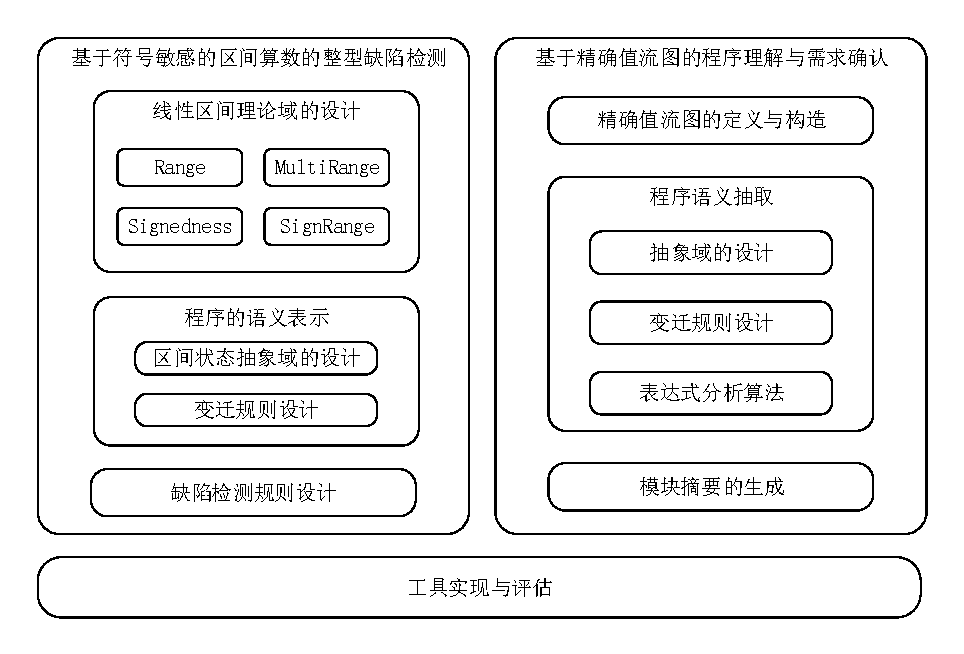
\includegraphics[width=6in]{YanJiuFangAn.pdf}
	\caption{研究方案}
	\label{fig:研究方案}
\end{figure}

  基于上述三点研究内容,本文提出如图\ref{fig:研究方案}所示的研究方案。
  
  \begin{enumerate}
  	\item 针对基于位敏感的区间代数的整型缺陷检测,本文进行如下三个方面的工作:其一是线性区间理论域的设计。为了增强现有区间抽象域表示能力和精度的不足,本文依次定义了线性区间Range、线性多区间MultiRange以及位敏感的线性多区间SignRange并设计了其计算规则。最后定义的SignRange能够较好的表示程序中整型变量的可能取值范围。其二,为了实现程序的语义表示,我们设计了区间状态抽象域RangeState来描述程序的每个状态,并通过定义变迁规则,模拟程序状态的变迁,从而实现程序的语义分析。最后,通过在RangeState上设计缺陷检测规则,实现程序的整型缺陷检测。
  	
  	\item 针对基于精确值流图的程序理解与需求确认,本文首先通过一个具体案例剖析使用基于值流图的程序理解方法为需求确认过程带来的好处,并以此展开,对该方法的具体内容做出了介绍。具体地,首先对精确值流图的定义与构造做出说明,基于精确值流图,设计了程序语义抽取方法。具体内容包括抽象域的设计、变迁规则的设计和表达式分析算法的设计。在上述的基础上,我们可以对程序整型变量在不同程序路径下的取值关系进行语义抽取。最后,利用得到的信息生成模块摘要。
  	
  	\item 最后,本文对上述两个研究方案中提出的方法进行编码实现,并设计相关实验,验证其正确性与实用性。
  \end{enumerate}
  
 
 \section{论文贡献}
 
 本文的贡献如下:
 \begin{enumerate}
 	\item 设计了表示能力更强的线性区间抽象域与变迁规则,使用它可以抽象表示程序在不同状态下整型变量的整数取值范围,进一步地,实现了针对C语言的整数缺陷检测方法;
 	
	\item 设计实现了一种基于内存模型的精准值流图分析构造方法,可处理动态内存空间、指针别名等传统数据流分析无法处理的语义关系,可区分数据流依赖、控制流依赖等依赖条件。同时,这一过程可自动化,并进一步可用于需求确认和缺陷分析,提升程序理解效率,提高代码质量;
	
	\item 基于上述两点,分别编码实现了相关工具并开展相关实验,证明了其正确性与实用性。
 \end{enumerate}
 
 \section{论文组织结构}
 
 本文的组织结构如下:
 
 第一章从软件验证与确认的角度介绍了整型缺陷分析与程序理解的相关背景知识与研究现状,并针对当前现状提出本文所研究内容与研究方案。
 
 第二章介绍了基于区间代数的整数缺陷检测方法,首先介绍了有关控制流自动机与可配置程序分析框架的基础知识,随后依次介绍扩展的整数(RangeInteger)、线性区间(Range)、线性多区间(MultiRange)和位敏感的线性多区间(SignRange)的理论域与计算规则的设计。我们以区间状态(RangeState)作为控制流自动机上状态节点的抽象表示,同时通过设计区间状态域上的变迁规则与整型缺陷检测规则,实现C语言上的整数缺陷检测。
 
 第三章介绍了基于精确值流图的程序理解与需求确认方法,首先通过一个机动车变速器控制逻辑的软件需求与实现的具体案例,介绍了程序理解对软件开发的重要性,并提出使用摘要来降低程序理解的难度。后续内容具体介绍了基于精确值流图的程序理解与需求确认方法的具体实现,包括抽象域、变迁规则的设计。在此基础上,介绍了变量关系分析方法、相关的程序理解方法与摘要的生成算法。
 
本文于第四章对上述问题的解决方法做了具体实现,并分别为两者设计了实验。通过实验验证了工具(算法)的有效性与实用性。随后,本文对实验中存在的误报、精度不足等问题做了具体分析并提出相关改进方案与技术展望。

第五章对本文所做工作进行了总结,并提出研究展望。
 
 
 
 
 
 
 
 
 
 
 
 
 
 
 
 
 
 
 
 
 
 
 
 
 
 
 
 
 
 
 
 
 
% !TeX root = ../main.tex

\chapter{基于区间代数的整数缺陷检测}
\label{sec:区间算数}

本章介绍基于区间代数的整数缺陷检测技术。旨在通过设计线性区间理论域,得到程序中整型变量的抽象表示,通过设计并借助变迁函数来模拟程序指令在抽象表示上的作用,实现程序的行为分析。在此基础上实现程序中数值导向型缺陷检测。

本章的结构安排如下:\ref{sec:区间算数引言}小节通过一个区间分析的案例,介绍了当前基于区间分析存在的精度不足问题,引出本章研究内容;\ref{sec:区间算数预备知识}小节介绍本章研究内容所需的预备知识,包括控制流自动机的概念与定义和可配置静态分析框架的概念;\ref{sec:区间算数抽象域设计}小节依照层次结构分别介绍了具体的线性区间理论域的设计,并介绍抽象域上的变迁函数;最后,本章\ref{sec:区间算数缺陷检测方法}小节利用设计的抽象域与变迁规则,给出程序的整型缺陷检测方法。我们于\ref{sec:WrappedRange}小节通过具体例子介绍环状区间,并以此展开,介绍未来可能的研究方向。

%最后于\ref{sec:区间算数模块实现}和\ref{sec:区间算数评估与结果}两个小节分别介绍了本章所述方法的工具实现并通过实验验证了工具的有效性。

\section{引言}
\label{sec:区间算数引言}

若要判定程序中整型变量所参与的计算是否可能产生整型溢出、除零异常及缓冲区溢出等缺陷,传统的解决方案是使用抽象解释将程序中的整型变量上近似抽象为1个整数区间。结合数据流分析,得到整型变量在整数区间抽象域上的近似值,并以此判定整型变量的操作是否安全。

尽管该方法能够在简单逻辑代码上得到较好的分析效果,但由于抽象域的表示能力有限,在程序的逻辑分支复杂的情况下,因状态合并操作所带来的精度损失较大,通常经过数次操作即到达抽象域的上界。

\begin{figure}[htb]
	\begin{subfigure}[b]{.5\linewidth}
			\begin{lstlisting}[xleftmargin=.15\textwidth]
void funcA(int i) {
	int x;
	if (i > 0) {
		x = funcB(i) - 5;
	} else {
		x = 5 - funcB(i);
	}
	assert(x != 0);
}
			\end{lstlisting}
%			\caption{A listing}
	\end{subfigure}
	\begin{subfigure}[b]{.5\linewidth}
			\begin{lstlisting}[xleftmargin=.25\textwidth]
int funcB(int i) {
	int x;
	if (i > 3) {
		x = 3 - i;
	} else {
		x = i;
	}
	return x;
}
			\end{lstlisting}
%		   (-∞, 3]
%			\caption{A listing}
\end{subfigure}
	\caption{基于区间代数的缺陷检测方法举例}
	\label{fig:codeExampleForSignRange}
\end{figure}{\tiny }

考虑图\ref{fig:codeExampleForSignRange}所示代码:函数A作为程序的入口,通过用户输入得到整型数值i,并根据i的大小使用不同的逻辑调用函数B并处理函数返回值。这里为讨论方便起见,规定int可表示所有整数值。若使用传统的基于整数区间抽象的数据流分析算法进行程序分析,易知函数B的返回值范围是$ [-\infty, 3] $,则函数A中第4行x的取值范围是$ [-\infty, -2] $,第6行x的取值范围是$ [2, +\infty] $。在第8行,由于状态合并,x的取值范围是$ [-\infty, +\infty] $,这将导致目标属性不成立。但实际上x的取值范围不包含0,目标属性是安全的。

为了解决上述问题,进一步提高程序分析的精度,本章提出了基于区间代数的整数缺陷检测技术,并在基于CPAchecker\cite{beyer2007configurable}的可配置的组合静态分析工具Tsmart上进行了实现。经过实验,基于本章工作实现的工具在Juliet测试集上的误报率小于3\%,漏报率为0\%。

\section{预备知识}
\label{sec:区间算数预备知识}

%\subsection{静态分析}
%
%静态分析是指在不运行代码的情况下,对程序源代码进行行为分析,从而判定程序是否满足某种特性。在代码的审查与优化、代码的缺陷分析与修复等方面有着大量应用。衡量静态分析技术的优劣通常考虑两个方面:分析精度和分析效率。分析精度用于衡量程序的实际行为与分析结果之间的匹配程度,分析效率则注重程序分析所消耗的资源大小,包括时间、存储的开销等。通常,程序分析的精度与效率是不可兼得的:分析精度的提高往往伴随着分析效率的下降,在实际应用中,我们往往需要平衡静态分析的精度与资源消耗,在不占用太多的资源下获得较好的分析精度一直是静态分析领域所重点关注的问题之一。

\subsection{控制流自动机}
\label{sec:控制流自动机}

控制流自动机(Control-flow Automaton,CFA)是命令式程序的一种语义等价表示方法,它是一个有向图:
\begin{definition}
	CFA可表示为有向图$ G = (N, E) $:$ N $是节点的集合,节点$ n \in N $表示程序的状态。$ E \subseteq N \times Ops \times N $是边的集合,有向边$ e = (n, op, n') \in E $表示从某个程序状态到下一个程序状态的过程,其中,$ Ops $是状态之间所执行的指令。一般地,我们用$ pred(e) $表示边$ e $的前驱节点$ n $,用$ succ(e) $表示边$ e $的后继节点$ n' $,用$ act(e) $表示边$ e $所执行的动作$ op $。
\end{definition}

在本文中,若无特殊说明,CFA是LLVM-IR语言上的等价表示,有向边$ e $根据其表示的指令的不同,可分为如下几类:
\begin{itemize}
	\item 空白边(BlankEdge):表示没有执行动作的边。即$ act(e) = \varepsilon $;
	
	\item 假设边(AssumeEdge):描述了假设条件是否成立。操作$ act(e) = (\%cmp, truth) $,其中$ \%cmp $为条件变量,它对应于LLVM-IR中i1类型的变量,表示假设条件。$ truth \in \{0, 1\}$为条件取值,表示当前边上假设条件变量$ \%cmp $的具体取值。一般地,我们用$ cond(e) $表示假设边的条件变量$ \%cmp $,用$ truth(e) $表示条件变量的取值$ truth $。
	
	\item Phi边(PhiEdge):描述了LLVM-IR中的phi指令。操作$ act(e) = (\%phi, index) $,其中$ \%phi $对应于phi指令,$ index $指示phi边上的第几个操作数作为当前指令的返回结果。
	
	\item 指令边(InstructionEdge):是CFA中最常见的边,描述了当前边执行了一条LLVM-IR指令。操作$ act(e) = (\%inst) $,其中$ \%inst $为所执行的指令。
	
%	\item 函数摘要边(FunctionSummaryEdge)

%	\item 函数调用边与函数返回边(FunctionCallEdge, FunctionReturnEdge):
\end{itemize}

为了便于后续算法介绍,我们对LLVM-IR中几种常见的指令做说明,现将其表示形式列举如下:
\begin{itemize}	
	\item Phi指令:$ z = \mathsf{phi}~[y_1, x_1]~ [y_2, x_2] \dots $。Phi指令通常具有多个输入$ [y_i, x_i] $,其中,$ y_i $表示可能的取值,$ x_i $用于表示取值条件,当程序的执行经过$ x_i $时,$ \mathsf{phi} $指令的取值对应为$ y_i $。
	
	\item Alloca指令:$ x = \mathsf{alloca}~type $。Alloca指令用于为变量$ x $申请一个能够存储类型为$ type $的内存区域,并将申请得到的内存地址返回给变量$ x $。
	
	\item 二元运算指令:$ x = y \cdot_{op} z $,$ \cdot_{op} \in \{+, -, \times, \div, and, or, xor, <<, >>\} $。二元运算指令用于对整型变量$ y, z $进行运算,并将计算结果赋值给$ x $。
	
	\item Cast指令:$ x = \mathsf{cast}~ y~ \mathsf{to}~type $。Cast指令用于将一个整型变量转化为类型为$ type $的整型变量。通常使用它转换整型变量的位宽。
	
	
	\item Cmp指令:$ x = \mathsf{cmp~pre}  ~y, z$。Cmp指令用于根据条件$ \mathsf{pre} $判定变量$ y $与$ z $的关系,并将比较结果返回给$ x $。判断条件$ \mathsf{pre} $通常有如下几种:
		\begin{itemize}
			\item eq: 判断$ y $与$ z $相等;
			\item ne: 判断$ y $与$ z $不相等;
			\item ugt: 无符号比较$ y > z $;
			\item uge: 无符号比较$ y \ge z $;
			\item ult: 无符号比较$ y < z $;
			\item ule: 无符号比较$ y \le z $;
			\item sgt: 有符号比较$ y > z $;
			\item sge: 有符号比较$ y \ge z $;
			\item slt: 有符号比较$ y < z $;
			\item sle: 有符号比较$ y \le z $。
		\end{itemize}
	
	\item Load指令:$ x = \mathsf{load} ~type ~y $。Load指令用于从$ y $所指向的内存区域中取类型为$ type $的数值,并将结果存放于变量$ x $中。
	
	\item Store指令:$ \mathsf{store}  ~type ~x, y $。Store指令用于将类型为$ type $的数值$ y $存放于由$ x $所指向的内存区域中。
\end{itemize}

为了便于描述,定义函数$ type $用于获取边的类型:
\begin{align}{\label{align:edgeType}}
	type(e) := \begin{cases}
		blank & e \in BlankEdge\\
		assume & e \in AssumeEdge\\
		phi & e \in PhiEdge\\
		inst & e \in InstructionEdge
	\end{cases}
\end{align}

\subsection{可配置程序分析框架} 
\label{sec:可配置程序分析框架}

可配置程序分析(Configurable Program Analysis,CPA)是一种通用的程序分析框架,通过设计并配置相关参数,实现在同一框架下完成多种不同的静态分析任务。通常,CPA框架将程序源代码转化为语义等价的控制流自动机并在CFA上多次应用静态分析算法实现程序分析。其中,CFA是源程序的等价表示,可描述为有向图。其节点表示指令位置、边表示控制流操作,如变量声明、运算、赋值、函数调用等。在分析时,我们常将内存地址抽象为内存位置,如访问路径\cite{cheng2000modular}等。

CPA算法的一次分析可表示为四元组$ \mathbb{D} = (D, \rightsquigarrow, merge, stop) $。其中,$ D $为抽象域;$ \rightsquigarrow $为转移关系,规定了在不同的控制流操作下,给定的抽象状态如何转移到新的抽象状态;$ merge $为状态合并算子;$ stop $为状态覆盖算子。

算法\ref{alg:CPA算法}描述了CPA的算法流程:算法以分析$ \mathbb{D}$、CFA图$ G $和初始状态$ e_0 \in E $作为输入,通过维护工作队列$ waitlist $和可达状态集$ R $并根据转移关系$ \rightsquigarrow $来计算当前状态$ e $的后继状态。工作队列和可达集的维护算法如算法\ref{alg:UpdateRW}所示,对每个后继状态$ e' $使用$ merge $算子来更新所有可达状态,如果可达状态$ e'' $被更新,则将该状态加入到等待队列$ waitlist $中以更新其后继状态。如果更新后的可达状态无法覆盖$ e' $,则将该状态分别加入$ waitlist $和可达集中。

\begin{breakablealgorithm}
	\caption{CPA算法}
	\label{alg:CPA算法}
	\begin{algorithmic}[1]
		
		\Require $ \mathbb{D} = (D, \rightsquigarrow, merge, stop) $,CFA图$ G $,初始状态$ e_0 \in E $
		\Ensure 可达状态集$ R $
		
		\State $ waitlist \gets \left\{ e_0 \right\} , R \gets \left\{ e_0 \right\}$
		\While{$ waitlist \ne \emptyset $}
			\State 取出$ waitlist $的首元素$ e $;
			\ForAll{$ e' $满足$ e \rightsquigarrow e' $}
				\State \Call{UpdateRW}{$ e', R, waitlist, merge, stop $};
			\EndFor
		\EndWhile
		
	\end{algorithmic}
\end{breakablealgorithm}

\begin{breakablealgorithm}
	\caption{UpdateRW算法}
	\label{alg:UpdateRW}
	\begin{algorithmic}[1]
		
		\Function{UpdateRW}{$ e', R, waitlist, merge, stop $}
			\ForAll{$ e' \in R $}
				\State $ e_{new}  \gets merge(e, e')$;
				\If{$ e_{new} \ne e' $}
					\State $ waitlist \gets (waitlist \cup \{e_{new}\}) \setminus \{e'\} $;
					\State $ R \gets (R \cup \{e_{new}\}) \setminus \{e'\} $;
				\EndIf
			\EndFor
			\If{$\neg stop(e, R)$}
				\State $ waitlist \gets (waitlist \cup \{e\}) $;
				\State $ R \gets R \cup \{e\} $;
			\EndIf
		\EndFunction
		
	\end{algorithmic}
\end{breakablealgorithm}

\section{基于线性空间的抽象域设计}
\label{sec:区间算数抽象域设计}

本节介绍基于线性空间的抽象域,其组成结构如图\ref{fig:Domains}所示。这里,位于最底层的是扩展的整数(RangeInteger)理论域,它是整数域的一个扩展,用于表示整型变量的某个可能取值。线性区间(Range)理论域表示整数区间,它是传统区间分析理论域的一个实现,以单独区间表示整型变量可能的取值范围。

在\ref{sec:区间算数引言}小节中,我们以图\ref{fig:codeExampleForSignRange}所示代码为例介绍了传统区间分析因区间个数问题所带来的精度丢失问题。为此,我们设计了线性多区间(MultiRange)理论域,它由若干个线性区间组成,具有更强的表示能力与更高的分析精度。更进一步地,面对具体的编程语言中整型变量所具有的位宽与符号性等属性,我们设计了位敏感的线性区间(SignRange)理论域,它是由线性多区间、位宽(Bitwidth)与符号性(Signedness)构成的三元组,使用SignRange可较好地刻画一个具有固定位宽的整型变量的可能取值范围,同时包含变量符号性信息。

在此基础上,我们引入区间状态(RangeState)抽象域,它描述了程序在某个状态下各个整型变量的取值信息,包括变量访问路径(AccessPath)、取值范围、符号性等。通过设计RangeState上的变迁关系(TransferRelation),我们可以得到程序在线性空间抽象域上的语义表示,为后续的整型缺陷分析提供支持。

\begin{figure}[H]
	\centering
	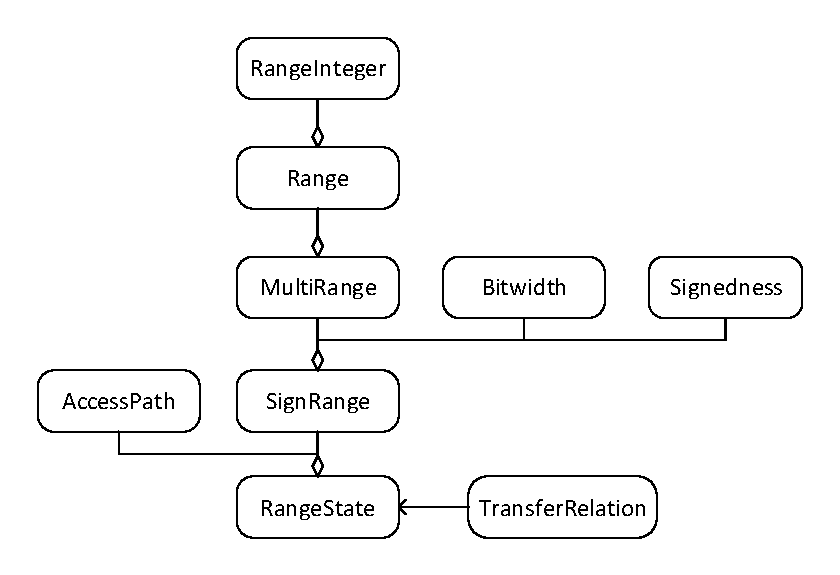
\includegraphics{Domains.pdf}
	\caption{抽象域的组成}
	\label{fig:Domains}
\end{figure}

\subsection{扩展的整数理论域}
\label{sec:Integer}

整型变量的可能取值是一个整数的集合,在这里我们使用扩展的整数RangeInteger来表示一个具体的整数,它是整数域$ \mathbf{Z} $的一个拓展。

\begin{definition}
	记$ D_I := \mathbf{Z} \cup \{ +\infty, -\infty, arb, nan\}  $为扩展的整数理论域。
	\begin{itemize}
		\item $ D_I $上的最大元($ \top_I $)为$ arb $,它表示任意值;最小元($ \bot_I $)为$ nan $,它表示非数;
		
		\item $ D_I $上的偏序关系($ \le_I $)为$ \mathbf{Z} $上的自然扩展,对于元素$ -\infty $与$ +\infty $,规定$ -\infty < +\infty $,且对任意$ x \in \mathbf{Z} $,有$ x < +\infty $以及$ -\infty < x $。特殊地,$ -\infty $与$ -\infty $、$ +\infty $与$ +\infty $无法比较,$ \bot_I, \top_I $与其他任意元素无法比较。
		
		\item $ D_I $上的上确界操作($ \sqcup_I $)定义为:\\
		\centerline{$ a \sqcup_I b := \begin{cases}
			\top_I & a \ne \bot_I \land b \ne \bot_I\\
			a & b = \bot_I\\
			b & a = \bot_I\\
			\bot_I & a = \bot_I \land b = \bot_I
			\end{cases} $}
	\end{itemize}
\end{definition}

对于元素$ -\infty $或$ +\infty $参与的运算,其规则如表\ref{tab:RangeInteger运算规则}所示。其中,函数$ signum $为取符号数,具体定义如下:
\begin{align}
	signum(x) := \begin{cases}
		1 & (x \in \mathbf{Z} \land x > 0) \lor x = +\infty\\
		0 & x = 0\\
		-1 & (x \in \mathbf{Z} \land x < 0) \lor x = -\infty
	\end{cases}
\end{align}

特别的,元素$ +\infty $与$ -\infty $所参与的某些运算是未定义的。这样的运算在表中记录为$ nan $,如$ (+\infty) +_I (-\infty), (+\infty) \div_I (+\infty)  $等。

\begin{longtable}{cclc}
	\caption[RangeInteger运算规则]{RangeInteger运算规则}
	\label{tab:RangeInteger运算规则}  \\ % add \\ command to tell LaTeX to start a new line	
	
	% Appear table header at the first page as well
	\toprule[1.5pt]	
	{\heiti 运算} & {\heiti 符号} & \multicolumn{1}{c}{\heiti 运算规则} \\
	\midrule[1pt]
	\endfirsthead
	
	% Appear the table header at the top of every page
	\multicolumn{3}{c}{续表~\thetable\hskip1em RangeInteger运算规则}\\
	\toprule[1.5pt]	
	{\heiti 运算} & {\heiti 符号} & \multicolumn{1}{c}{\heiti 运算规则} \\
	\midrule[1pt]
	\endhead 
	
	% Appear \hline at the bottom of every page
	\hline
	\multicolumn{3}{r}{续下页}
	\endfoot 
	\endlastfoot
	
	% data begins here				
		negate & $ neg_I $ & $  neg_I(x) :=  \begin{cases}
			-x & x \ne \pm\infty\\
			-\infty & x = +\infty\\
			+\infty & x = -\infty\\
		\end{cases}$\\
		
		add &$  +_I $ & $ x +_I y :=  \begin{cases}
			x + y & x, y \ne \pm\infty\\
			x & x = \pm\infty \land y \ne \pm\infty\\
			y & x \ne \pm\infty \land y = \pm\infty\\
			x & x, y = \pm\infty \land signum(x) = signum(y) \\
			nan & \text{其他}
		\end{cases}$ \\
		
		subtract & $ -_I $ & $ x -_I y := \begin{cases}
			x - y & x, y \ne \pm\infty\\
			x & x = \pm\infty \land y \ne \pm\infty\\
			neg(y) & x \ne \pm\infty \land y = \pm\infty\\
			x & x, y = \pm\infty \land signum(x) \ne signum(y) \\
			nan & \text{其他}
		\end{cases} $\\
		
		multiply & $ \times_I $ & $ x \times_I y := \begin{cases}
			x \times y & x, y \ne \pm\infty\\
			+\infty & signum(x) \times signum(y) > 0\\
			-\infty & signum(x) \times signum(y) < 0\\
			nan & \text{其他}
		\end{cases} $\\
		
		\begin{tabular}{c}
			divide\\
			$ (y \ne 0) $\\
		\end{tabular} & $ \div_I $ & $ x \div_I y := \begin{cases}
			x \div y & x, y \ne \pm\infty\\
			0 & x \ne \pm\infty \land y = \pm\infty\\
			+\infty \times_I signum(x \times_I y) & x = \pm\infty \land y \ne \pm\infty\\				
			nan & \text{其他}
		\end{cases} $\\
		
		\begin{tabular}{c}
			modular\\
			$ (y > 0) $\\
		\end{tabular} & $ mod_I $ & $ x \mod_I y := \begin{cases}
		x \mod y & x, y \ne \pm\infty\\
		x & x \ge 0 \land y = +\infty\\
		y & x < 0 \land y =+\infty\\
		nan & \text{其他}
		\end{cases} $\\
		
		\begin{tabular}{c}
			and\\
			or\\
			xor\\
			shl\\
			shr
		\end{tabular} & \begin{tabular}{c}
		$ and_I $\\
		$ or_I $\\
		$ xor_I $\\
		$ <<_I $\\
		$ >>_I $
	\end{tabular} & $ x \cdot_{op_I} y := \begin{cases}
		x \cdot_{op} y & x, y \ne \pm\infty\\
		nan & \text{其他}
		\end{cases} $\\
	
	% more data here
	\bottomrule[1.5pt]
\end{longtable}

\subsection{线性区间理论域}
\label{sec:Range}

线性区间Range是一个整数区间,表示整型变量的可能取值范围。它是由两个整数$ x, y $构成的二元组。这里,$ x, y $为扩展的整数域RangeInteger上的元素,其定义与偏序关系定义如下。

\begin{definition}
	线性区间理论域$ D_R :=  \{ [x, y] | x \in \mathbf{I}, y \in \mathbf{I}, x \le y \} \cup \{ \emptyset \}$是一个半格:	
	\begin{itemize}
		\item $ D_R $上的最大元($ \top_R $)是$ [-\infty, +\infty] $,最小元($ \bot_R $)是空集$ \emptyset $;
		\item $ D_R $上的偏序关系($ \le_R $)定义为:\\	
		\centerline{$ [x_1, y_1] \le_R [x_2, y_2] \iff x_2 \le x_1 \land y_1 \le y_2 $;}
		\item $ D_R $上的上确界操作($ \sqcup_R $)定义为:\\	
		\centerline{$ [x_1, y_1] \sqcup_R [x_2, y_2] := [\min(x_1, x_2), \max(y_1, y_2)] $,}  \\
		此处$ \max $和$ \min $为$ D_I $上的自然扩展。
	\end{itemize}
\end{definition}

我们在Range上定义一些基础的运算操作,其运算规则如表\ref{tab:Range运算规则}所示。值得注意的是,最小元$ \bot_R $与任何元素的计算结果均为$ \bot_R $,为表示方便,在表中默认操作数均不为$ \bot_R $。

\begin{longtable}{cclc}
	\caption[Range运算规则]{Range运算规则}
	\label{tab:Range运算规则}  \\ % add \\ command to tell LaTeX to start a new line	
	
	% Appear table header at the first page as well
	\toprule[1.5pt]	
	{\heiti 运算} & {\heiti 符号} & \multicolumn{1}{c}{\heiti 运算规则} \\
	\midrule[1pt]
	\endfirsthead
	
	% Appear the table header at the top of every page
	\multicolumn{3}{c}{续表~\thetable\hskip1em Range运算规则}\\
	\toprule[1.5pt]	
	{\heiti 运算} & {\heiti 符号} & \multicolumn{1}{c}{\heiti 运算规则} \\
	\midrule[1pt]
	\endhead 
	
	% Appear \hline at the bottom of every page
	\hline
	\multicolumn{3}{r}{续下页}
	\endfoot 
	\endlastfoot
	
	% data begins here	
	negate & $ neg_R $ & $  neg_R([x, y]) := [[neg_I(x), neg_I(y)]]_R$\\
	
	add & $ +_R $ & $ [x_1, y_1] +_R [x_2, y_2] := [[x_1 +_I x_2, y_1 +_I y_2]]_R $\\
	
	subtract & $ -_R $ & $ [x_1, y_1] -_R [x_2, y_2] :=  [[	x_1 -_I y_2, y_1 -_I x_2]]_R$\\
	
	multiply & $ \times_R $ & \begin{tabular}{lc}
		$ [x_1, y_1] \times_R [x_2, y_2] := $\\
		$ [\min(vals), \max(vals)], vals = \{x_1, y_1\} \times_{\times_I} \{x_2, y_2\} $
	\end{tabular}\\

	\begin{tabular}{c}				
		divide\\
		$ (op_2 \ne 0)$
	\end{tabular}& $ \div_R $ & \begin{tabular}{lc}
		$  [x_1, y_1] \div_R [x_2, y_2] := $ \\
		$ \begin{cases}
			[\min(vals), \max(vals)] &\begin{tabular}{lc}
				$ 0 \notin [x_2, y_2]$,  \\
				$ vals = \{x_1, y_1\} \times_{\div_I} \{x_2, y_2\}  $
			\end{tabular}\\
			[x_1, y_1] \div_R [1, y_2] & x_2 = 0\\
			[x_1, y_1] \div_R [x_2, -1] & y_2 = 0\\
			[neg(upper), upper] & \begin{tabular}{lc}
				$ x_2 < 0 < y_2,  $ \\
				$ upper = \max(|x_1|, |y_1|) $
			\end{tabular}\\
		\end{cases} $
	\end{tabular}\\

	\begin{tabular}{c}
		modular\\
		$ (op_2 \ne 0) $\\
	\end{tabular} & $ mod_R $ & \begin{tabular}{lc}
		$ [x_1, y_1] \mod_R [x_2, y_2] := $ \\
		$ \begin{cases}
			op_1 -_R op_2 \times_R times_1 & \begin{tabular}{lc}
				$ x_2 > 0 $\\
				$ times_1 = op_1 \div_R op_2 +_R [1, 1] $
			\end{tabular}\\
			
			op_1 -_R op_2 \times_R times_2 & \begin{tabular}{lc}
			$ y_2 < 0 $\\
			$ times_2 = op_1 \div_R op_2 -_R [1, 1] $
			\end{tabular}\\
		\end{cases} $
	\end{tabular}\\

	\begin{tabular}{c}
		and\\
	\end{tabular} & $ and_R $ & \begin{tabular}{lc}
		$ [x_1, y_1]\  and_R \ [x_2, y_2] := $ \\
		$ \begin{cases}
			x_1 \ and_I \ y_1 & x_1 = y_1 \land x_2 = y_2\\
			[0, y_1] & x_1 = y_1 \ge 0\\
			[0, y_2] & x_2 = y_2 \ge 0\\
			[0, +\infty] & x_1 \ge 0 \lor x_2 \ge 0\\
			[-\infty, -1] & y_1 < 0 \land y_2 < 0\\
			[-\infty, +\infty] & \text{其他}
		\end{cases} $
	\end{tabular}\\
	
	\begin{tabular}{c}
		or\\
	\end{tabular} & $ or_R $ & \begin{tabular}{lc}
		$ [x_1, y_1] \ or_R \  [x_2, y_2] := $ \\
		$ \begin{cases}
			x_1 \ or_I \  y_1 & x_1 = y_1 \land x_2 = y_2\\
			[-1, -1] & x_1 = y_1 = -1 \lor x_2 = y_2 = -1\\
			[\max(x_1, x_2), +\infty] & x_1 \ge 0 \land x_2 \ge 0\\
			[-\infty, -1] & y_1 < 0 \lor y_2 < 0\\
			[-\infty, +\infty] & \text{其他}
		\end{cases} $
	\end{tabular}\\

	\begin{tabular}{c}
		xor\\
	\end{tabular} & $ xor_R $ & \begin{tabular}{lc}
		$ [x_1, y_1] \ xor_R \  [x_2, y_2] := $ \\
		$ \begin{cases}
			x_1 \ xor_I \  y_1 & x_1 = y_1 \land x_2 = y_2\\
			[x_1, y_1] & x_2 = y_2 = 0\\
			[x_2, y_2] & x_1 = y_1 = 0\\
			[-\infty, +\infty] & x_1 \times_I x_2 < 0 \lor x_2 \times_I x_2 < 0\\
			[0, +\infty] & (x_1 \ge 0 \land x_2 \ge 0) \lor (y_1 < 0 \land y_2 < 0)\\
			[-\infty, -1] & \text{其他}
		\end{cases} $
	\end{tabular}\\

	\begin{tabular}{c}
		shl\\
	\end{tabular} & $ <<_R $ & \begin{tabular}{lc}
		$ [x_1, y_1] <<_R  [x_2, y_2] := $ \\
		$ \begin{cases}
			\emptyset & y_2 < 0\\
			[x_1, y_1] <<_R [0, y_2] & 0 \in [x_2, y_2]\\
			[\min(vals), \max(vals)] & \text{其他,} vals = \{x_1, y_1\} \times_{<<_I} \{x_2, y_2\}
		\end{cases} $
	\end{tabular}\\

	\begin{tabular}{c}
		shr\\
	\end{tabular} & $ >>_R $ & \begin{tabular}{lc}
		$ [x_1, y_1] >>_R  [x_2, y_2] := $ \\
		$ \begin{cases}
		\emptyset & y_2 < 0\\
		[x_1, y_1] >>_R [0, y_2] & 0 \in [x_2, y_2]\\
		[\min(vals), \max(vals)] & \text{其他,}vals = \{x_1, y_1\} \times_{>>_I} \{x_2, y_2\}
		\end{cases} $
	\end{tabular}\\
	% more data here
\bottomrule[1.5pt]
\end{longtable}

在表格中,我们定义了构造函数$ [[\cdot]]_R $,利用它可以方便的构造Range:
\begin{align}
[[x, y]]_R := \begin{cases}
[x, y] & x, y \text{是可比较的,且}  x \le y\\
[y, x] & x, y \text{是可比较的,且}  x > y\\
\emptyset & \text{其他}
\end{cases}
\end{align}

同时,为了进一步简化书写,我们定义了集合上的操作$ \times_{\cdot_{op}} $。对集合$ setA $和$ setB $,有:
\begin{align}
setA  \times_{\cdot_{op}} setB =  \{ e_i \cdot_{op} e_j \, | \, e_i \in setA, e_j \in setB \} 
\end{align}

Range是可比较的,对于$ a = [x_1, y_1], b = [x_2, y_2] \in D_R $,有:
\begin{align}
	a < b \iff y_1 < x_2\\
	a > b \iff x_1 > y_2
\end{align}

\subsection{线性多区间理论域}
\label{sec:MultiRange}

通过分析图\ref{fig:codeExampleForSignRange}所示的代码案例,易知在整型变量分析时,使用单独的线性区间Range会造成一定程度的精度损失,这时需要提供一个更为精确的理论域来对整型变量的取值范围做抽象。

本小节介绍线性多区间MultiRange,它是由0到$ L_{MR} $个Range构成的有序的区间列表,通过使用多个Range区间,MultiRange能够提供更贴近实际域的变量取值区间表示。当$ L_{MR}  \rightarrow \infty $时,MultiRange能够精确表示整型变量的每一个可能取值,其表示能力和RangeInteger相同;当$ L_{MR} = 1 $时,MultiRange的表示能力与Range相同。

在实际应用中,由于MultiRange可以根据需要通过改变$ L_{MR} $值的大小灵活改变理论域的表示精度,从而可以十分灵活的针对不同情况,优化程序分析的分析效率与分析精度。

\begin{definition}
	线性多区间理论域$ D_{MR}  := \{ [r_1, \dots, r_n] \ | \ r_i \in D_R,  r_1 < \dots < r_n, 0 \le n \le L_{MR} \}$是一个半格:
	\begin{itemize}
		\item $ D_{MR} $上的最大元($\, \top_{MR} $)是$ [\top_R] $,最小元(\, $ \bot_{MR} $ ) 是$ [\,] $;
		
		\item $ D_{MR} $上的偏序关系($ \le_{MR} $)定义为:\\
			\centerline{$[a_1, \dots, a_m] \le_{MR} [b_1, \dots, b_n] \iff$}
			\centerline{$ \forall \ a_i, \ \exists\  b_j \text{ 使得} \ a_i \le_R b_j .\  (0 \le i \le m, 0 \le j \le n)$;}
			
		\item $ D_{MR} $上的上确界操作($ \sqcup_{MR} $)定义为:\\
			\centerline{$ [a_1, \dots, a_m] \sqcup_{MR} [b_1, \dots, b_n]  := $}
			\centerline{$ [[a_1, \dots, a_m, b_1, \dots, b_n]]_{MR} .\  (0 \le i \le m, 0 \le j \le n)$。}
	\end{itemize}
	
\end{definition}

上述的定义中使用了MultiRange的构造函数$ [[\cdot]]_{MR} $,其函数逻辑如算法\ref{alg:MultiRange}所示。该函数接受一个由Range组成的集合$ ranges $或直接给出待组合的Range列表$ range_1, range_2, \dots, range_n $。首先根据每个区间的左值和右值进行排序,得到有序的Range列表$ ranges $。并将$ ranges $中所有相互包含或相邻的区间进行合并,得到有序的且不互相包含、连接的区间列表$ nRanges $。为了保证得到的MultiRange中Range的个数小于$ L_{MR} $,在算法结束前不断合并前后相邻的且距离最小的Range直至其个数满足要求。

\begin{breakablealgorithm}
	\caption{MultiRange的构造器$ [[\cdot]]_{MR} $}
	\label{alg:MultiRange}
	\begin{algorithmic}[1]
		
		\Require $ ranges = \{range_1, \dots, range_n\}, L_{MR} $
		\Ensure $ [nRange_1, \dots, nRange_m]. \ (0 \le m \le L_{MR})$
		
		\State sort $ ranges $ by $ range_{i}.x $ then by $ range_{i}.y $
		\State $ nRanges \gets \emptyset$
		\State $ [low, high] \gets$ peek$ (ranges) $
		\ForAll{$ range_i $ in $ ranges $}
			\If{$ range_i.x \le high +_I 1 $}
				\State $ high \gets \max(range_i.y, high) $
			\Else
				\State $ nRanges \gets nRanges \cup [low, high] $
				\State $ [low, high] \gets range_i $
			\EndIf
		\EndFor
		\While{$ size(nRanges) > L_{MR} $}
			\State pick range pair $ (nRange_i, nRange_{i+1} )$ in $ nRanges $ whose distance is shortest
			\State $ nRanges \gets (nRanges \setminus\{nRange_i, nRange_{i+1}\}) \cup (nRange_i \sqcup_R nRange_{i+1}) $
			\State sort $ nRanges $ by $ nRange_{i}.x $ then by $ nRange_{i}.y $
		\EndWhile
		\\\Return $ toList(nRanges) $
		
	\end{algorithmic}
\end{breakablealgorithm}

我们同样在MultiRange上定义一些基础运算操作,如表\ref{tab:MultiRange运算规则}所示。为方便起见,记$ r = [r_1, \dots, r_n] $为一个MultiRange,它是一个有序Range列表。我们在MultiRange上沿用定义在集合上的符号$ \times_{\cdot_{op}} $,即对于$ a, b \in D_{MR}$,有$ a \times_{\cdot_{op}} b = toList(set_{\cdot_{op}}) $,其中$ set_{\cdot_{op}} = \{a_i \cdot_{op} b_j \, | \, a_i \in a, b_j \in b\, , 0 \le i \le m, 0 \le j \le n\}$。

\begin{longtable}[H]{ccc}
	\caption[MultiRange运算规则]{MultiRange运算规则}
	\label{tab:MultiRange运算规则}  \\ % add \\ command to tell LaTeX to start a new line	
	
	% Appear table header at the first page as well
	\toprule[1.5pt]	
	{\heiti 运算} & {\heiti 符号} & \multicolumn{1}{c}{\heiti 运算规则} \\
	\midrule[1pt]
	\endfirsthead
	
	% Appear the table header at the top of every page
	\multicolumn{3}{c}{续表~\thetable\hskip1em MultiRange运算规则}\\
	\toprule[1.5pt]	
	{\heiti 运算} & {\heiti 符号} & \multicolumn{1}{c}{\heiti 运算规则} \\
	\midrule[1pt]
	\endhead 
	
	% Appear \hline at the bottom of every page
	\hline
	\multicolumn{3}{r}{续下页}
	\endfoot 
	\endlastfoot
	
	% data begins here	
	negate & $ neg_{MR} $ & $  neg_{MR}(r) :=[[neg_R(r_1), \dots, neg_R(r_n)]]_{MR}$\\
	
	add & $ +_{MR} $ & \begin{tabular}{lc}
		$ a +_{MR} b  :=  [[a \times_{+_R} b]]_{MR}$
	\end{tabular}\\
	
	subtract & $ -_{MR} $ & \begin{tabular}{lc}
		$ a -_{MR} b  :=  [[a \times_{-_R} b]]_{MR} $
	\end{tabular}\\
	
	multiply & $ \times_{MR} $ & \begin{tabular}{lc}
		$ a \times_{MR} b :=  [[a \times_{\times_R} b]]_{MR} $
	\end{tabular}\\
	
	\begin{tabular}{c}				
		divide
	\end{tabular}& $ \div_{MR} $ & \begin{tabular}{lc}
		$ a \div_{MR} b :=   [[a \times_{\div_R} b]]_{MR}, \, b \ne 0$
	\end{tabular}\\
	
	\begin{tabular}{c}
		modular\\
	\end{tabular} & $ \mod_{MR} $ & \begin{tabular}{lc}
		$ a \mod_{MR}  \,  b :=   [[a \times_{\mod_R} b]]_{MR}, \, b \ne 0 $
	\end{tabular}\\
	
	\begin{tabular}{c}
		and\\
	\end{tabular} & $ and_{MR} $ & \begin{tabular}{lc}
		$ a  \,  and_{MR} \,   b :=  [[a \times_{and_R} b]]_{MR} $
	\end{tabular}\\
	
	\begin{tabular}{c}
		or\\
	\end{tabular} & $ or_{MR} $ & \begin{tabular}{lc}
		$ a  \,  or_{MR}  \,  b :=  [[a \times_{or_R} b]]_{MR} $
	\end{tabular}\\
	
	\begin{tabular}{c}
		xor\\
	\end{tabular} & $ xor_{MR} $ & \begin{tabular}{lc}
		$ a  \,  xor_{MR} \,   b :=  [[a \times_{xor_R} b]]_{MR} $
	\end{tabular}\\
	
	\begin{tabular}{c}
		shl\\
	\end{tabular} & $ <<_{MR} $ & \begin{tabular}{lc}
		$ a <<_{MR} b :=  [[a \times_{<<_R} b]]_{MR} $
	\end{tabular}\\
	
	\begin{tabular}{c}
		shr\\
	\end{tabular} & $ >>_{MR} $ & \begin{tabular}{lc}
		$ a >>_{MR} b :=  [[a \times_{>>_R} b]]_{MR} $
	\end{tabular}\\
	% more data here
	\bottomrule[1.5pt]
\end{longtable}

由于MultiRange是由Range组成的有序列表,通过观察表\ref{tab:MultiRange运算规则}易知,其计算规则是Range计算规则的简单拓展。考虑两个只含有单独区间的MultiRange:$ a = [[1, 3]]$,$ b = [[2, 3]] $。$ a \times_{MR} b $按照上述计算规则的计算结果为$ [[1, 3] \times_R [2, 3]]  = [[2, 9]] $,而实际上$ a \times_{MR} b $的取值不可能为$ 5, 7, 8 $,计算存在精度丢失。为了解决上述问题,在后续章节提出优化方案,可进一步提升MultiRange的计算精度。

MultiRange是可比较的,对于$ a = [a_1, \dots, a_m], b = [b_1, \dots, b_n] \in D_{MR}$,有:
\begin{align}
	a < b \iff a_m < b_1\\
	a > b \iff a_1 > b_m
\end{align}

为了后续便利,在MultiRange上定义如下函数:
\begin{itemize}
	\item $ kill(mr, r) = mr \setminus r, mr \in D_{SR}, r \in D_R$用于删除$ sr $所表示的整数范围中$ r $对应的部分。例如:
	对于$ mr = [[0, 255]] $,有$ mr.kill([10, 100]) = [[0, 9],  [101, 255]] $。
	
	\item $ join(mr, r) = mr \cap r, mr \in D_{SR}, r \in D_R $用于得到$ mr $所表示的整数范围中与$ r $重合的部分。例如:
	对于$ mr = [[1, 10], [20, 30]] $,有$ mr.join([5, 25]) = [[5, 10], [20, 25]] $。
\end{itemize}

\subsection{位敏感的线性区间理论域}
\label{sec:SignRange}

在前面介绍的RangeInteger、Range与MultiRange抽象表示均未考虑整型变量在计算机上的存储格式,即对变量在计算机中所占用字节的大小是不敏感(Bitwidth Sensitive)的。当程序分析需要考虑变量的字节大小时,这类抽象表示往往不能提供整型变量实际所能表示的整数范围。

位敏感的线性区间SignRange = (MultiRange, Bitwidth, Signedness)是一个三元组。其中,MultiRange是上小节所述的线性多区间;Bitwidth表征了变量在计算机中所占用的位宽;Signedness表征了存储于计算机中整型变量在程序中是以有符号还是无符号的形式解析的。

\begin{definition}
	符号性(Signedness)理论域$ D_{sgn} := \{Signed, Unsigned, Unknown\} $是一个半格:
	\begin{itemize}
		\item $ D_{sgn} $上的最大元($ \top_{sgn} $)是$ Unsigned $,最小元($ \bot_{sgn} $)是$ Unknown $;
		
		\item $ D_{sgn} $上的偏序关系($ \le_{sgn} $)定义为:\\
			\centerline{$ Unknown \le_{sgn} Signed \le_{sgn} Unknown $}
			
		\item $ D_{sgn} $上的上确界操作($ \sqcup_{sgn} $)定义为:\\
			\centerline{$ s_1 \sqcup_{sgn} s_2 := \begin{cases}
				s_2 & s_1 \le_{sgn} s_2\\
				s_1 & s_2 \le_{sgn} s_1\\
				\end{cases} $}
	\end{itemize}
\end{definition}

引入符号性理论域意味着一个整型变量取值范围会随着符号性的不同而映射为不同的SignRange,尽管其在计算机内的存储内容是相同的(解释方式不同)。由于程序的这一特点,定义函数$ |_{to}(s), s \in D_{sgn} $用于转化同一整数取值范围的不同SignRange表示,其算法在后续给出。方便起见,可将$ Signed, Unsigned, Unknown $分别记为$ S, U, N $。在此之前,先定义位敏感的线性区间SignRange的理论域:

\begin{definition}
	位敏感的线性区间理论域	$ D_{SR} := \{(r, w,  s) \, | \,  r \in D_{MR}, w \in \mathbf{Z^+}, s \in \{Signed, Unsigned, Unknown\}\} $是一个半格:
	\begin{itemize}
		\item $ D_{SR} $上的最大元($ \top_{SR} $)是$ (\top_{MR}, \top_{Z^+}, s) $,最小元($ \bot_{SR} $)是$ (\bot_{MR}, \bot_{\mathbf{Z}^+}, s)$;
		
		\item $ D_{SR} $上的偏序关系($ \le_{SR} $)定义为:\\
			\centerline{$ (r_1, w_1, s_1) \le_{SR} (r_2, w_2, s_2) \iff (r_1 \,  |_{to}(\mathsf{s}(r_2)) \le_{MR} r_2) \land (w_1 \le w_2) $;}
			
		\item $ D_{SR} $上的上确界操作($ \sqcup_{SR} $)定义为:\\
			\centerline{$ (r_1, w_1, s_1) \sqcup_{SR} (r_2, w_2, s_2)  :=  (r, w, s) , $其中,$ \begin{cases}
				s := \max(s_1, s_2)&\\
				w := \max(w_1, w_2)&\\
				r := r_1 |_{to}(s) \sqcup_{MR} r_2 |_{to}(s)&\\
				\end{cases}$。}
	\end{itemize}
\end{definition}

上述定义中,函数$ \mathsf{s}(sr), sr \in D_{SR}$用于取位敏感线性区间$ sr $的Signedness值。类似的,有$ \mathsf{w}(sr), sr \in D_{SR} $用于取区间$ sr $的Bitwidth值;$ \mathsf{r}(sr), sr \in D_{SR} $用于取区间$ sr $的MultiRange值。


值得注意的是,$ \mathsf{r}(\top_{SR}) := \top_{MR} $。这意味着在SignRange中MultiRange的实际可取值范围比计算机表示范围大,这一特性将用于程序分析判定整型变量是否产生整型溢出。为了表示在计算机上固定位宽的整型变量的实际取值范围,定义函数$ top(sr), sr \in D_{SR} $和函数$ top(w, s), w \in \mathbf{Z^+}, s \in D_{sgn} $用于计算在特定位宽下的整型变量以特定符号性解释的取值范围:
\begin{align}
	top(sr)  = top(w, s):=  \begin{cases}
		[0, 2^{w} - 1]_{R} & s = U\\
		[-2^{w - 1}, 2^{w - 1} - 1]_{R} & s \in \{S, N\}
	\end{cases}
\end{align}

作为补充的,定义函数$ bound(sr), sr \in D_{SR}$和$ bound(sr, w, s), sr \in D_S, w \in \mathbf{Z^+}, s \in D_{sgn}  $用于得到取值范围在限定范围内的SignRange:
\begin{align}
	bound(sr) := (sr \cap top(sr), \mathsf{w}(sr), \mathsf{s}(sr))\\
	bound(sr, w, s) := (sr|_{to}(s) \cap top(w, s), w, s)
\end{align}

函数$ |_{to} $的转换规则如算法\ref{alg:toUnsigned}和算法\ref{alg:toSigned}。

\begin{breakablealgorithm}
	\caption{Convert2Unsigned, $ |_{to}(U) $}
	\label{alg:toUnsigned}
	\begin{algorithmic}[1]
		
		\Require $ signRange = (ranges, bitwidth, signedness) , signedness \in \{S, N\}$
		\Ensure new SignRange with Unsigned type
		
		\State $ convertVal \gets top(bitwidth, Unsigned).y + 1 $
		\State $ nRanges \gets \emptyset $
		\ForAll{$ range $ in $ range(signRange) $}
			\If{$ range < 0 $}
				\State $ nRanges \gets nRanges \cup (range +_R convertVal) $
			\ElsIf{$ range > -1 $}
				\State $ nRanges \gets nRanges \cup range $
			\Else
				\State $ nRanges \gets nRanges \cup ([range.x, -1] +_R convertVal) \cup [0, range.y] $
			\EndIf
		\EndFor
		\\\Return $ nSignRange = ([[nRanges]]_{MR}, bitwidth, Unsigned) $
	\end{algorithmic}
\end{breakablealgorithm}

\begin{breakablealgorithm}
	\caption{Convert2Signed, $ |_{to}(S) $}
	\label{alg:toSigned}
	\begin{algorithmic}[1]
		
		\Require $ signRange = (ranges, bitwidth, signedness) , signedness \in \{U, N\}$
		\Ensure new SignRange with Signed type
		
		\State $ topVal \gets top(bitwidth, Signed) $
		\State $ convertVal \gets top(bitwidth, Unsigned).y + 1 $
		\State $ nRanges \gets \emptyset $
		\ForAll{$ range $ in $ range(signRange) $}
			\If{$ range < topVal + 1 $}
				\State $ nRanges \gets nRanges \cup range $
			\ElsIf{$ range > topVal $}
				\State $ nRanges \gets nRanges \cup (range -_R convertVal) $
			\Else
				\State $ nRanges \gets nRanges \cup [range.x, topVal] $
				\State $ nRanges \gets nRanges \cup ([topVal + 1, range.y] -_R convertVal) $
			\EndIf
		\EndFor
		\\\Return $ nSignRange = ([[nRanges]]_{MR}, bitwidth, Signed) $
	\end{algorithmic}
\end{breakablealgorithm}

与MultiRange相比,SignRange的计算规则着重考虑符号性。一般地,二元操作符在运算前需要统一其左右操作数的符号性。如无特殊说明,对操作数$ a, b \in D_{SR}$参与的二元运算$ a \cdot_{op} b $将按如下规则(Unifiy Signedness)更新自己的符号性并进行运算:

(1)当$ \cdot_{op} \in \{add, subtract, multiply, divide, mod\} $时,按下列规则更新符号性、位宽并运算:
\begin{align}{\label{align:Unify规则}}
	w' = \mathsf{w}(a) = \mathsf{w}(b) \gets \max(\mathsf{w}(a), \mathsf{w}(b)) \\
	a \cdot_{op} b := \begin{cases}
		a |_{to}(U) \cdot_{op} b |_{to}(U) & \mathsf{s}(a) = U \lor \mathsf{s}(b) = U\\
		a \cdot_{op} b & \mathsf{s}(a) = N \land \mathsf{s}(b) = N\\
		a |_{to}(S) \cdot_{op} b |_{to}(S) & \text{其他}
	\end{cases}
\end{align}

(2)当$ \cdot_{op} \in \{and, or, xor\} $时,按下列规则运算,不更新位宽与符号性:
\begin{align}
	a \cdot_{op} b := a |_{to}(S) \cdot_{op} b |_{to}(S)
\end{align}

(3)当$ \cdot_{op} \in \{shl, shr\} $时,按下列规则更新符号性并运算,不更新位宽:
\begin{align}
	a \cdot_{op} b := a \cdot_{op} b |_{to}(U)
\end{align}

SignRange的计算规则如表\ref{tab:SignRange计算规则}所示。由于多数二元运算的操作数在运算前要更新符号性与位宽,因此表\ref{tab:SignRange计算规则}中若如无特殊说明,计算结果中的$ w' \in \mathbf{Z^+}, s' \in D_{sgn} $均为操作数按照Unify Signedness规则统一符号性、位宽后得到的值。


\begin{longtable}{ccc}
	\caption[SignRange运算规则]{SignRange运算规则}
	\label{tab:SignRange计算规则}  \\ % add \\ command to tell LaTeX to start a new line	
	
	% Appear table header at the first page as well
	\toprule[1.5pt]	
	{\heiti 运算} & {\heiti 符号} & \multicolumn{1}{c}{\heiti 运算规则} \\
	\midrule[1pt]
	\endfirsthead
	
	% Appear the table header at the top of every page
	\multicolumn{3}{c}{续表~\thetable\hskip1em SignRange运算规则}\\
	\toprule[1.5pt]	
	{\heiti 运算} & {\heiti 符号} & \multicolumn{1}{c}{\heiti 运算规则} \\
	\midrule[1pt]
	\endhead 
	
	% Appear \hline at the bottom of every page
	\hline
	\multicolumn{3}{r}{续下页}
	\endfoot 
	\endlastfoot
	
	% data begins here	
	negate & $ neg_{SR} $ & \begin{tabular}{lc}
		$ neg_{SR}(r) :=  \begin{cases}
		(neg_{MR}(\mathsf{r}(r)), \mathsf{w}(r), \mathsf{s}(r)) & \mathsf{s}(r) \in \{S, N\}\\
		neg_{SR}(r \, |_{to}(S)) \, |_{to}(U) & s = U\\
		\end{cases}$
		
	\end{tabular}\\
	
	add & $ +_{SR} $ & $ a +_{SR} b := (\mathsf{r}(a) +_{MR} \mathsf{r}(b), w', s') $\\
	
	subtract & $ -_{SR} $ & $ a -_{SR} b := (\mathsf{r}(a) -_{MR} \mathsf{r}(b), w', s') $\\
	
	multiply & $ \times_{SR} $ & $ a \times_{SR} b := (\mathsf{r}(a) \times_{MR} \mathsf{r}(b), s', s') $\\
	
	\begin{tabular}{c}				
		divide\\
	\end{tabular}& $ \div_{SR} $ & $ a \div_{SR} b := (\mathsf{r}(a) \div_{MR} \mathsf{r}(b), w', s'), b \ne 0 $\\
	
	\begin{tabular}{c}
		modular\\
	\end{tabular} & $ \mod_{SR} $ & \begin{tabular}{c}
		$ a \mod_{SR} \, b := (\mathsf{r}(a) \mod_{MR} \, \mathsf{r}(b), w', s'), b \ne 0 $
	\end{tabular}\\
	
	\begin{tabular}{c}
		and\\
	\end{tabular} & $ and_{SR} $ & \begin{tabular}{c}
		$ a \, and_{SR} \, b := (\mathsf{r}(a) \, and_{MR} \, \mathsf{r}(b), \mathsf{w}(a), \mathsf{s}(a)) $
	\end{tabular}\\
	
	\begin{tabular}{c}
		or\\
	\end{tabular} & $ or_{SR} $ & \begin{tabular}{c}
		$ a \, and_{SR} \, b := \mathsf{r}(a) \, or_{MR} \, \mathsf{r}(b), \mathsf{w}(a), \mathsf{s}(a)) $
	\end{tabular}\\
	
	\begin{tabular}{c}
		xor\\
	\end{tabular} & $ xor_{SR} $ & \begin{tabular}{c}
		$ a \, and_{SR} \, b := (\mathsf{r}(a) \, xor_{MR} \, \mathsf{r}(b), \mathsf{w}(a), \mathsf{s}(a)) $
	\end{tabular}\\
	
	\begin{tabular}{c}
		shl\\
	\end{tabular} & $ <<_{SR} $ & \begin{tabular}{c}
		$ a <<_{SR} b :=  (\mathsf{r}(a) <<_{MR} \mathsf{r}(b'), \mathsf{w}(a), s'),  $\\
		$ \quad\quad\quad \text{in which } b' \gets b.kill([\mathsf{w}(a), +\infty]).kill([-\infty, -1])$
	\end{tabular}\\
	
	\begin{tabular}{c}
		shr\\
	\end{tabular} & $ >>_{SR} $ & \begin{tabular}{c}
		$ a <<_{SR} b := (\mathsf{r}(a) >>_{MR} \mathsf{r}(b'), \mathsf{w}(a), s'),  $\\
		$ \quad\quad\quad \text{in which } b' \gets b.kill([\mathsf{w}(a), +\infty]).kill([-\infty, -1])$
	\end{tabular}\\
	% more data here
	\bottomrule[1.5pt]
\end{longtable}

在上一小节中,我们提到MultiRange在某些操作下会产生一定的精度丢失,这些精度丢失将会在后续章节进行修正。本节介绍的SignRange由于是MultiRange的扩展,其计算规则大部分调用了MultiRange的计算规则,因此对MultiRange的精度优化可以不加修改的继承到SignRange。

需要注意的是,由于SignRange是位敏感的,因此在进行shl和shr操作时,其计算精度仍可优化,优化方法将在后续章节随MultiRange的优化一同给出。

SignRange是可比较的,对于$ a, b \in D_{SR} $,有:\begin{align}
	a < b \iff \mathsf{r}(a') < \mathsf{r}(b')\\
	a > b \iff \mathsf{r}(a') > \mathsf{r}(b')
\end{align}

其中,$ a', b' $为根据Unify Signedness规则(\ref{align:Unify规则})更新符号性和位宽后得到的SignRange。

为了后续方便,在SignRange上定义函数$ high $用于获取当前线性区间中的最大值,函数$ low $用于获取当前线性区间中的最小值。对于$ sr = ([[1, 5], [20, 100]],8,\\ S) \in D_{SR} $,有$ high(sr) = 100, low(sr) = 1 $。

\subsection{区间状态理论域}
\label{sec:RangeState}

通过上一小节的分析,使用位敏感的线性区间SignRange可以对整型变量的取值范围做精确的抽象表示和计算模拟,本节介绍的区间状态RangeState则是对控制流自动机(CFA)中所表示的程序状态的精确抽象,它描述了CFA上某程序状态下各个整型变量的取值范围。

区间状态RangeState := AccessPath $ \mapsto $ SignRange是一个从AccessPath到SignRange的映射,用符号$ \Gamma $表示。它描述了在某个程序状态下,所有通过访问路径AccessPath访问得到的整型变量的可能取值范围SignRange。其中,AccessPath描述了一个整型变量在内存中的访问路径,通过这个访问路径,可以得到整型变量在内存中的唯一表示。若AccessPath的理论域为$ D_{ap} $,那么对于$ x \in D_{ap}$,记$ \Gamma(x) $为$ x $在$ \Gamma $上的映射,即访问路径为$ x $的位敏感的线性区间表示。

对于一个待分析程序,我们在其等价表示CFA上定义理论域$ D_{S} $:

\begin{definition}
	定义区间状态理论域$ D_S  := \{\Gamma := x \mapsto y ~|~ x \in D_{ap}, y \in D_{SR}  \}  $是一个半格:
	\begin{itemize}
		\item $ D_S $上的最大元$ \top_S  := x \mapsto \top_{SR}, x \in D_{ap} $,最小元$ \bot_S := x \mapsto \bot_{SR}, x \in D_{ap} $;
		
		\item $ D_S $上的偏序关系($ \le_S $)定义为:\\
		\centerline{$ a \le_S b \iff \mathsf{aps}(a) \subseteq \mathsf{aps}(b) \, \land  \forall x \in \mathsf{aps}(a), a(x) \le_{SR} b(x) $;}
		
		\item $ D_S $上的上确界操作($ \sqcup_S $)定义为:\\
		\centerline{$ a \sqcup_S b :=  x \mapsto y , x \in \mathsf{aps}(a)  \cup  \mathsf{aps}(b), y = a(x) \sqcup_{SR} b(x)  $。}
	\end{itemize}
\end{definition}

上述定义中,函数$ \mathsf{aps}(\Gamma) := \{x \in D_{ap}~|~ \Gamma(x) \ne \bot_{SR}\} $ 表示区间状态$ \Gamma $的访问路径集合。类似的,定义函数$ \mathsf{ranges}(\Gamma) := \{ \Gamma(x) ~|~x \in \mathsf{aps}(x) \} $为取状态区间$ \Gamma $的区间表示SignRange的集合。

区间状态$ \Gamma $通常与CFA上的状态节点$ n $是关联的,本节定义的区间状态RangeState是对控制流自动机CFA中节点$ n $上整型变量取值信息的精确抽象。根据章节\ref{sec:控制流自动机}中的定义,CFA的边$ e $表示从一个程序状态到下一个程序状态的过程,$ act(e) $表示边$ e $所执行的动作。对应的,我们定义理论域$ D_S $上的变迁关系$ \rightsquigarrow_S $为CFA的边$ e $所表示的程序变迁关系的抽象:
\begin{definition}
	记$ \rightsquigarrow_S := D_S \times Ops \times D_S $为区间状态理论域$ D_S $上的变迁关系。其中,$ Ops $表示变迁关系上的操作。	我们用$ \Upsilon := act(\rightsquigarrow_S) $来表示$ Ops $所具体执行的动作,称之为变迁函数。对于$ s \in D_S $,$ s' = \Upsilon(s) $表示区间状态$ s $在应用变迁函数$ \Upsilon $后得到的新的区间状态。
\end{definition}

在定义区间状态理论域上的变迁关系后,我们可以使用区间状态$ \Gamma $和区间状态上的变迁关系$ \rightsquigarrow_S $来抽象描述CFA上程序状态和程序状态之间的变迁关系。由于CFA上对应的边$ e \in E $所表示的指令类型的不同(见公式\ref{align:edgeType}),$ \rightsquigarrow_S $对应的变迁函数$ \Upsilon := act(\rightsquigarrow_S) $随之有不同的定义(下列定义中为方便起见,整型变量的AccessPath均由其在指令中的变量名代替):

\begin{enumerate}

\item 对于空白边$ e \in BlankEdge $,$ act(e) = \varepsilon $,其变迁关系为:
\begin{align}
	\frac{n_1 \xrightarrow{\varepsilon} n_2, S_2 = S_1}{(n_1, S_1) \to (n_2, S_2))}
	\quad\textsf{T-R-EMPTY}
\end{align}

其中,$ n_1, n_2 \in N $表示CFA上的状态节点,$ S_1, S_2 $则为$ n_1, n_2 $在区间状态域$ D_S $上的抽象表示。为方便起见,如无特殊说明,后续定义中的$ n_1, n_2, S_1, S_2 $同此含义。

\item 对于假设边$ e \in AssumeEdge $,$ act(e) = (\%cmp, truth) $。其中,$ truth \in \{true, false\} $。其变迁关系为:
\begin{align}
	\frac{n_1 \xrightarrow{[\%cmp = truth]} n_2, 
		S_2 = \mathsf{refineVals}(S_1, \%cmp, truth)}
	{(n_1, S_1) \to (n_2, S_2)}
	\quad\textsf{T-R-ASSUME}
\end{align}

其中,函数$ \mathsf{refineVals} $的操作是将区间状态$ S_1 $中访问路径为$ \%cmp $的取值范围改为$ truth $所代表的值,同时依照比较逻辑更改比较操作的两个操作数的范围。

\item 对于形如$ z = \mathsf{phi}~[y_1, x_1]~[y_2, x_2] $的Phi边(PhiEdge),其变迁关系为:
\begin{align}
\frac{n_1 \xrightarrow{z = \mathsf{phi}~[y_1, x_1]~[y_2, x_2] } n_2, 
	S_2 = S_1[z ~/~ Y ]}
{(n_1, S_1) \to (n_2, S_2)}
\quad\textsf{T-R-PHI}
\end{align}

在上式中,当$ S_1(x_1) = 0 $时,$ Y := 	S_1(y_1) $ 当 $ S_1(x_2) = 0 $时,$ Y :=  S_1(y_2) $。

\item 对于形如$ x = \mathbf{alloca}  ~type $这样的指令边(InstructionEdge),约定$ w $为$ type $类型变量在计算机上存储所用位宽,$ s $为$ type $类型变量的符号性,则变迁关系可描述为:
\begin{align}
	\frac{n_1 \xrightarrow{x = \mathbf{alloca}  ~type} n_2, 
		S_2 = S_1[*x ~/~ (\top_{MR}, w, s) ]}
	{(n_1, S_1) \to (n_2, S_2)}
	\quad\textsf{T-R-ALLOCA}
\end{align}

\item 对于形如$ x = y \cdot_{op} z $这样的指令边,其变迁关系为:
\begin{align}
	\frac{n_1 \xrightarrow{x = y \cdot_{op} z} n_2, 
		S_2 = S_1[x ~/~ S_1(y) \cdot_{op_{SR}} S_1(z) ]}
	{(n_1, S_1) \to (n_2, S_2)}
	\quad\textsf{T-R-OP}
\end{align}

此处$ \cdot_{op_{SR}} $为$ \cdot_{op} $在$ D_{SR} $上的自然扩展。

\item 对于形如$ x = \mathsf{cast}  ~y ~\mathsf{to} ~type$这样的指令边,其变迁关系为:
\begin{align}
\frac{n_1 \xrightarrow{x = \mathsf{cast}  ~y ~\mathsf{to} ~type} n_2, 
	S_2 = S_1[x ~/~ bound(S_1(x), w, s) ]}
{(n_1, S_1) \to (n_2, S_2)}
\quad\textsf{T-R-CAST}
\end{align}

其中,$ w $为$ type $类型变量在计算机上存储所用位宽,$ s $为$ type $类型变量的符号性。后续定义中,若无特殊说明,对于指令中出现的$ type $类型,将继续沿用符号$ w, s $。

\item 对于形如$ x = \mathsf{cmp~pre}  ~y, z$这样的指令边,其变迁关系为:
\begin{align}
\frac{n_1 \xrightarrow{x = \mathsf{cmp~pre}  ~y, z} n_2, 
	S_2 = S_1[x ~/~ \mathsf{compare}(S_1(y), S_1(z)) ]}
{(n_1, S_1) \to (n_2, S_2)}
\quad\textsf{T-R-CMP}
\end{align}

其中,函数$ \mathsf{compare}(a, b), a, b\in D_{SR} $用于在$ D_{SR} $上依据定义的比较规则得到的比较结果。

\item 对于形如$ x = \mathsf{load} ~type ~y $这样的指令边,其变迁关系为:
\begin{align}
\frac{n_1 \xrightarrow{x = \mathsf{load}  ~y } n_2, 
	S_2 = S_1[x ~/~ bound(S_1(*y), w, s)]}
{(n_1, S_1) \to (n_2, S_2)}
\quad\textsf{T-R-LOAD}
\end{align}

\item 对于形如$ \mathsf{store}  ~type ~x, y $这样的指令边,其变迁关系为:
\begin{align}
\frac{n_1 \xrightarrow{\mathsf{store}  ~type ~x, y} n_2, 
	S_2 = S_1[*y ~/~ bound(S_1(x), w, s)]}
{(n_1, S_1) \to (n_2, S_2)}
\quad\textsf{T-R-STORE}
\end{align}

\end{enumerate}

\subsection{精度优化}

在\ref{sec:MultiRange}和\ref{sec:SignRange}小节中,通过举例我们知道,对于两个单独的区间在进行乘法、位移等操作时会产生一定程度的精度丢失。而造成精度丢失的原因是,单独区间如$ r = [x, y] $只能描述从$ x $到$ y $的全部整数。而乘法、位移等操作会拉大区间内整数之间的距离,从而导致精度的丢失。

为了解决这一问题,我们于\ref{sec:MultiRange}小节提出了线性多区间的概念,它定义了一个由多个线性区间组成的列表,可以更加精确的表示整数的取值范围。但是在定义MultiRange的乘法等运算时,其运算规则仅仅是组合调用Range的运算规则,并没有深入优化Range与Range之间计算的精度。

借助MultiRange本身即可表示多个区间这一良好的性质,理想情况下我们可以将线性区间所表示的所有整数打散并分别进行运算,再重新将计算结果组合为多区间列表。例如,对于$ a = [[1, 3]] \in D_{MR} , b = [[2, 3]] \in D_{MR}$两个线性区间,我们可将其分别表示为$ a' = \{1, 2, 3\}, b' = \{2, 3\} $。则区间上的运算$ a \times_{MR} b $的运算结果可以通过集合上的运算结果$ a' \times_{\times_I} b' = \{2, 3, 4, 6, 9\} $导出,则$ a \times_{MR} b = [[2, 4], [6, 6], [9, 9]] $。

以上思路实际上是线性区间在具体域上的运算还原。其计算过程实际上是对整型变量的所有可能取值的枚举,这违背了抽象解释技术的初衷。在具体应用中,变量的可能取值范围通常是很大的,仅区间$ x = [[1, 10], [20, 100]] $即表示了90个可能的整数取值。由此可知,当区间与区间进行运算时,尽管枚举区间的所有可能取值并分别运算提高了分析的精度,但也伴随着分析效率的极大下降。

为了兼顾分析效率与分析精度,本节给出的优化方法的主要思想是在合理的区间长度下将区间打散并对区间内每个整数分别进行运算,当区间内包含的整数过多时,直接进行原始的区间运算。这样做的原因基于整型变量在程序中的使用通常符合如下几类情况:
\begin{itemize}
	\item 作为输入变量,通过条件判断语句逐步缩小并确认整型变量的可表示范围;
	\item 作为普通变量参与运算,变量初始化时可能通过常量赋值也可能通过变量复制赋值。
\end{itemize}

其中,本节提出的优化的具体应用多针对于取值范围很小的变量,如上述情形中的通过常量(如常数、枚举值等)赋值初始化的整型变量、通过比较操作得到的布尔型变量、以及具体出现的小区间范围的变量等。

我们在MultiRange上补充定义函数$ exsits $,对于一个整数$ x \in D_R $和线性区间$ mr \in D_{MR} $,$ mr.exsists(x) $用于判定$ mr $中是否存在整数$ x $;定义$ \mathsf{cnt}(mr) $用于获取$ mr $表示的线性区间内包含的整数个数;定义函数$ \mathsf{disperse}(mr) := \{r = [x, x] \in D_R ~|~ mr.exsits(x) \}$用于得到$ r $对应的整数表示集合。

则对于MultiRange上二元运算$ z := x \cdot_{op} y$,其中$ \cdot_{op} \in \{ multiply, and, or, xor, \\shl, shr \} $,其优化后的运算规则可表述为:
\begin{align}
	x \cdot_{op} y := \begin{cases}
		[[\mathsf{disperse}(x) \times_{\cdot_{op_R}} \mathsf{disperse}(y)]]_{MR} & 
			\mathsf{cnt}(x), \mathsf{cnt}(y) \le L_{MR}\\
		x \cdot_{op} y & \text{其他}
	\end{cases}
\end{align}

其中,操作符$ \cdot_{op_R} $为操作符$ \cdot_{op} $在理论域$ D_R $上的对应版本。另一方面,在位敏感的线性区间SignRange上,由于其计算规则的定义是MultiRange的扩展,因此无需修改,直接应用优化后的计算规则即可。


\section{基于区间代数的整数缺陷检测方法}
\label{sec:区间算数缺陷检测方法}

整型缺陷按照类型通常可分为两类:一类是数值型缺陷,这包括比如整型的上溢出、下溢出、整型的除零异常等;另一类是由数值型缺陷所引发的其他类型缺陷。典型的如内存泄漏、缓冲区溢出等。这类问题相较于单纯的数值型缺陷往往危害更大。以上两类缺陷可统称为数值导向型缺陷。

其中,整型的溢出缺陷是由程序变量在计算机中有限长度的二进制表示造成的。例如,在C语言中,一个类型为$ signed ~int $的变量在计算机上通常存储为32位二进制数,这意味着该变量的表示是有范围的。当欲表达的整型数字超过表达的最大范围,就会出现整型溢出。由于C语言中对溢出的行为是未定义的,部分机器对上溢出的数字解释为负数,由此可能会出现潜在的程序逻辑紊乱。

上述数值导向型缺陷均可在标准错误枚举(Common Weakness Enumeration,简称CWE)中找到定义,如表\ref{tab:CWE}所示。


\begin{longtable}{p{1cm}p{5.5cm}p{7cm}}
	\caption[CWE定义的数值导向型缺陷]{CWE定义的数值导向型缺陷}
	\label{tab:CWE}  \\ % add \\ command to tell LaTeX to start a new line	
	
	% Appear table header at the first page as well
	\toprule[1.5pt]	
	{\heiti 编号} & {\heiti CWE类型} & {\heiti 解释} \\
	\midrule[1pt]
	\endfirsthead
	
	% Appear the table header at the top of every page
	\multicolumn{3}{c}{续表~\thetable\hskip1em CWE定义的数值导向型缺陷}\\
	\toprule[1.5pt]	
	{\heiti 编号} & {\heiti CWE类型} & {\heiti 解释} \\
	\midrule[1pt]
	\endhead 
	
	% Appear \hline at the bottom of every page
	\hline
	\multicolumn{3}{r}{续下页}
	\endfoot 
	\endlastfoot
	
	% data begins here	
	190 & Integer Overflow or Wraparound & 整数运算的结果小于数学算术期望值\\
	191 & \begin{tabular}{lc}
		Integer Underflow \\
		(Wrap or Wraparound) 
	\end{tabular}& 整数运算的结果大于数学算术期望值\\
	126 & Buffer Overread & 缓冲区读取位置超过缓冲区上界\\
	127 & Buffer Underread & 缓冲区读取位置未达到缓冲区下界\\
	121 & Stack-based Buffer Overflow & 对超出栈内存对象上界的位置写入数据\\
	122 & Heap-based Buffer Overflow & 对超出堆内存对象上界的位置写入数据\\
	124 & Buffer Underflow & 对未达到内存对象下界的位置写入数据\\
	369 & Divide by Zero & 除零异常\\
	401 & Memory	Leak& 堆内存泄露\\	
	% more data here
	\bottomrule[1.5pt]
\end{longtable}

本节介绍的基于区间代数的整型缺陷检测方法可直接应用于检测数值型缺陷,即表\ref{tab:CWE}中所对应的CWE-190、CWE-191和CWE-369。对于由数值型缺陷导致的其他缺陷,可使用本节提出的方法配合其他CPA算法加以实现。

在小节\ref{sec:RangeState}中,我们介绍了控制流自动机CFA的抽象表示RangeState以及其上与CFA边对应的状态变迁关系。本节所述的缺陷检测算法实际上是区间状态RangeState抽象域的一个具体应用。要检测程序是否出现整型溢出、除零异常等缺陷,我们要在原有的区间状态变迁规则基础上,设计缺陷检测规则。

通过分析,易知如需检测整型的溢出和除零异常缺陷,仅需关注程序中的整型变量在二元运算或位宽转换指令时的状态即可。

对于CFA上通过边$ e $连接的两个状态节点$ n_1, n_2 $。当$ e $是形如$ x = y \cdot_{op} z $ ,其中 $\cdot_{op} \in \{ add, subtract, multiply, shl, shr \} $这样的操作边(InstructionEdge)时,我们对其应用上溢出和下溢出检测规则:
\begin{align}
	\label{align:overflow}\mathsf{isOverflow}(n_1, e) \iff top(X) < high(X), X = S_1(y) \cdot_{op_{SR}} S_1(z)\\
	\label{align:underflow}\mathsf{isUnderflow}(n_1, e) \iff low(X) < top(X), X = S_1(y) \cdot_{op_{SR}} S_1(z)
\end{align}

其中,操作符$ \cdot_{op_{SR}} $是操作符$ \cdot_{op} $在SignRange上的对应版本。$ S_1, S_2 $是状态节点$ n_1, n_2 $在区间状态理论域$ D_S $上的抽象表示。类似的,当 $\cdot_{op} \in \{ divide, mod \} $时,我们应用除零检测规则:
\begin{align}
	\label{align:dividebyzero}\mathsf{isDivideByZero}(n_1, e) \iff X.exsists(0), X = S_1(y) \cdot_{op_{SR}} S_1(z)
\end{align}

其中,函数$ exsists $为MultiRange上的自然扩展。我们将上述检测规则描述为算法\ref{alg:checkEdge}。对CFA上的每条边,应用checkEdge判定其是否存在整型缺陷,并生成缺陷报告。

\begin{breakablealgorithm}
	\caption{checkEdge for CWE190, 191 and 369}
	\label{alg:checkEdge}
	\begin{algorithmic}[1]
		
		\Require $ e \in E, n_1, n_2 \in N$,其中$ e $是CFA中连接节点$ n_1, n_2 $的有向边
		
		\If{$ type(e) = inst \land act(e) = \cdot_{op} $}
		
			\If{$ \cdot_{op} \in \{add, subtract, multiply, shl, shr \} \land \mathsf{Wrapped}$ is false }
				\If{$ \mathsf{isOverflow(n_1, e)} $}
					\State report an IntegerOverflow weakness at $ (n_1, e) $
				\ElsIf{$ \mathsf{isUnderflow(n_1, e)} $}
					\State report an IntegerUnderflow weakness at $ (n_1, e) $
				\EndIf
			\EndIf
			
			\If{$ \cdot_{op} \in \{divide, mod\} \land \mathsf{isDivideByZero(n_1, e)}$}
				\State report a DivideByZero weakness at $ (n_1, e) $
			\EndIf
		
		\EndIf
				
	\end{algorithmic}
\end{breakablealgorithm}

上述算法中,$ \mathsf{Wrapped} $符号来自LLVM-IR指令,对应于二元运算中的NSW与NUW符号,用于表征运算是否允许因运算上溢出、下溢出所带来的数值翻转。

\section{环状区间理论域简介}
\label{sec:WrappedRange}

尽管本章提出的位敏感线性区间抽象域SignRange能够精确表示整型变量的可能取值范围,但在具体编码实现中会相对复杂。本节将用少量篇幅介绍环状区间WrappedRange,它将作为本章未来的研究内容。

在\ref{sec:SignRange}小节中,为了实现对整型变量符号性的表示,我们引入了符号性Signedness与位敏感区间SignRange来扩充现有线性区间在表示性上的不足,并在此基础上实现了对程序状态的抽象表示。但实际上这样的区间设计存在着一定程度的冗余,原因是一个整型变量不论是有符号数还是无符号数,其在计算机上的存储模式是一致的:同一个二进制串既可以按有符号数来解析,又可以按无符号数来解析。但对于SignRange而言,同一个整型变量对应的二进制串按其符号性解析方式不同,对应着两个不同的SignRange。这一方面造成了表示性的冗余,增加静态分析所用的内存,另一方面也增加了编码实现的难度。

为了解决这一问题,本节介绍一种线性区间表示的替代方案——环状区间WrappedRange\cite{navas2012signedness, gange2015interval},它最早由Navas等人于2012年提出。环状区间的实现思路基于整型变量在计算机中的二进制表示与解析,它实质上模拟了以二进制串存储的整型变量在计算机中的表示与操作。它解决了SignRange对同一个整型变量因符号性不同而产生的不同抽象解释,一定程度上降低了编码实现的难度。

我们以一个具体例子介绍WrappedRange的运作方式,其形式化的定义与详细的计算规则将作为本文的未来研究工作内容,这里不做具体论述。

环状区间通常可表示为由两个长度为$ w $的二进制向量$ x, y $构成的二元组$ [x, y] $。其中,二进制向量$ x, y $可理解为整型数字在计算机中的存储模式。例如,对于$ x = 1001 $表示位宽为4的整型数字,它既可以按有符号数解释为-7,又可按无符号数解释为9。

那么,对于一个环状区间$ r = [x, y] ~($ 其中 $x, y \in \{0, 1\}^w $ 且 $ x \ne y + 1) $,它所表示的具体整数取值范围是:
\begin{align}
	r = [x, y] := \begin{cases}
	\{x, \dots, y\} & x \le y\\
	\{0^w, \dots, y\} \cup \{x, \dots, 1^w\} & \text{其他}
	\end{cases}
\end{align}

为了便于对环状区间的理解,我们以长度$ w = 4$的向量构成的环状区间为例介绍环状区间的性质与运算。如图\ref{fig:wrappedRange}所示,将$ \{0, 1\}^w $所表示的向量以环状形式排列,则环状区间$ r = [x, y], x, y\in \{0, 1\}^4, x \ne y + 1 $所表示的取值可理解为图\ref{fig:wrappedRange}上以$ x $为起点,以$ y $为终点顺时针访问得到的所有向量。

例如,对于$ r = [0110, 1001] $,其表示范围是$ \{0110, 0111, 1000, 1001\} $,对应有符号数为$ \{6, 7, -8, -7\} $,对应的无符号数为$ \{6, 7, 8, 9\} $。由于区间是环状定义的,因此允许区间的左值大于右值,对应的其区间为图\ref{fig:wrappedRange}中超过180°的扇形区域。例如$ r = [1101, 0001] $的表示范围是$ \{1101, 1110, 1111, 0000, 0001 \} $,对应的有符号数为$ \{-3, -2, -1, 0, 1\} $,对应的无符号数为$ \{13, 14, 15, 0, 1\} $。

那么,对于环状区间$ r_1 = [x_1, y_1], r_2 = [x_2, y_2] $,其加法规则可以表述如下:
\begin{align}
	r_1 + r_2 = \begin{cases}
	[x_1 + x_2, y_1 + y_2] & \mathsf{len}(r_1) + \mathsf{len}(r_2) \le 2^w\\
	[0^w, 1^w] & \text{其他}
	\end{cases}
\end{align}

类似地,我们可在未来进一步完善环状区间相关的计算规则。

\begin{figure}[htb]
	\centering
	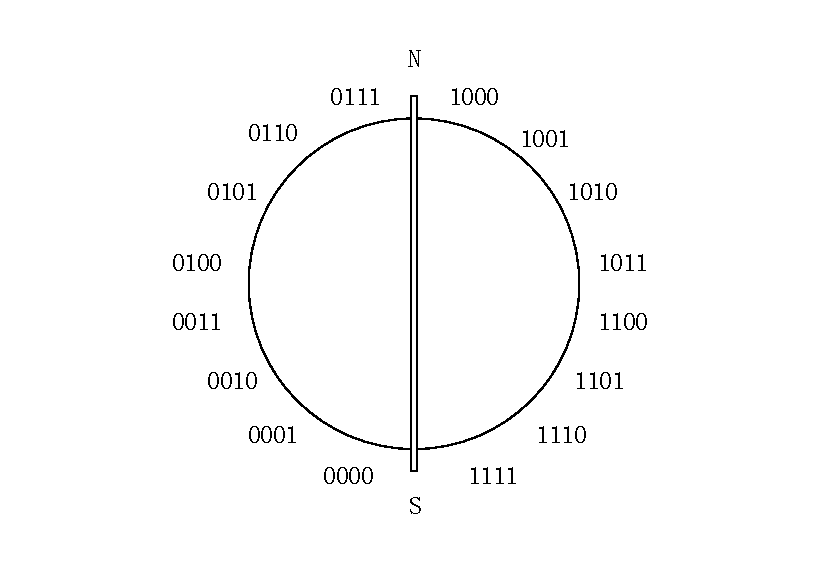
\includegraphics{WrappedRange.pdf}
	\caption{以环状形式列出的所有$ \{0, 1\}^4 $元素}
	\label{fig:wrappedRange}
\end{figure}

通过环状区间,我们可以将有符号数、无符号数统一进行表示。但与线性区间Range相同地,它们均面临着无法精细刻画多段区间的情形。在后续工作中,我们将会进一步研究基于环状区间WrappedRange的多区间理论域,进一步提升其表示能力。

\section{本章小结}

本章介绍了基于区间代数的整型缺陷分析方法,其核心是理论域的设计。本章先介绍了整体的区间设计,随后依次对各个抽象层面进行介绍,并结合控制流自动机,设计了整型变量的缺陷检测规则。最后,在基于Tsmart-V3静态分析框架上做了实现,并通过实验验证了其有效性。

在\ref{sec:Integer}小节,我们介绍了扩展的整数RangeInteger,相比于整数,其具体定义了$ +\infty $和$ -\infty $的概念,同时,我们介绍了有$ -\infty, +\infty $参与的整数运算规则,为后续介绍区间抽象域奠定了基础。在\ref{sec:Range}小节,介绍了基于扩展整数的区间Range,它以单独区间的形式表示了一个整型变量的可能取值范围,并首次定义整数区间上的运算规则。

随后,在\ref{sec:MultiRange}和\ref{sec:SignRange}小节,我们介绍了线性多区间MultiRange与位敏感的线性多区间SignRange,它们的提出分别解决了单独的Range区间精度不足以及无法描述符号性的问题。随后为了进一步提升多区间在区间长度较小时的精度,提出了基于拆分-合并思想的精度提升方法。

最后,结合CPA,提出了基于区间代数的缺陷检测方法。该方法基于区间状态RangeState抽象域,它是CFA上程序状态节点的抽象。通过设计抽象域与变迁规则,可以得到整型变量在程序指令执行前后的取值区间,从而实现整型缺陷分析。在第\ref{sec:值流图评估与结果}章节,我们将通过实验,验证基于区间代数的缺陷检测方法的有效性。

值得一提的是,本章设计的位敏感的线性多区间SignRange是对整型变量的具体含义做抽象,其并未反应变量在计算机中的实际存储。实际上,针对存储于计算机上的0-1二进制串,我们以有符号数和无符号数对其进行解析时会得到两个不同的SignRange抽象表示,这会给该理论域的具体编程实现带来一定的困难,并造成一定程度的表示冗余。为了解决这一问题,本章于\ref{sec:WrappedRange}介绍了环状区间的概念,并希望以此解决上述问题。该理论域的具体实现与优化将作为今后研究的方向。





















































% !TeX root = ../main.tex

\chapter{基于值流图的整型变量关系分析与缺陷检测}

本章介绍基于值流图的整型变量关系分析与缺陷检测方法,该方法的核心是快速、自动化的从代码中抽取出程序语义,建立程序实现与需求之间的关系,帮助开发人员理解程序进行需求确认。

本章结构安排如下:\ref{sec:值流图引言}小节简要归纳了当前程序理解技术,提出本章工作的实际意义与必要性;\ref{sec:值流图案例分析}小节通过一个需求与实现的例子具体介绍了本章工作如何帮助开发人员快速进行软件确认;随后\ref{sec:值流图程序理解方法}小节具体介绍了算法的原理与实现方法,并于\ref{sec:值流图评估与结果}小节进行了实验验证。\ref{sec:值流图总结}小节最后对本章工作做了总结。

\section{引言}
\label{sec:值流图引言}

软件验证与确认是软件研发过程中十分重要的步骤。其中,对软件确认过程来说,人们除了使用测试的手段逐条对软件行为进行验证以外,最常用的手段便是在理解程序代码的基础上对程序是否符合软件需求做判断。但是,在条件分支众多、代码逻辑复杂的情况下,现有工具很难帮助用户理清程序输入输出变量之间的关系。文章\inlinecite{maalej2010can}指出,约25\%的代码维护工作流程是发现问题-修改-再验证的,同时,大量的开发者通过假设并验证程序的行为来理解软件\cite{maalej2014comprehension}。因此,若使用一种算法(工具)帮助开发者快速准确地抽取程序语义将会大大减少程序理解相关工作时间。

程序理解\cite{boysen1979factors, sackman1968exploratory}领域以往的研究工作主要基于程序切片技术、程序标记技术以及执行可视化技术。

程序切片技术\cite{binkley1996program}本质上是一种代码拆解技术。它通过剔除与指定变量不相关的代码语句,一定程度上减少了用户的代码阅读量。但是由于其并未能给出更上层的程序语义,用户仍需要阅读源码以获取知识。与之相反,程序标记技术\cite{sulir2017labeling}通过在源码上附加辅助信息的方式来帮助用户理解代码。现有工具可提供的辅助信息多种多样,但本质上用户仍要理解代码逻辑,并不能显著提升程序理解速度。执行可视化工具使用动态分析获取程序的执行信息并将之可视化,为了达到分析目的,工具将不同执行过程信息加以融合。其缺点是当程序逻辑复杂时,可视化的效果会变差,且需要为其配置程序运行环境,具有上手难度。 

本章中,我们提出了一种基于精确值流图(Value Flow Graph,简称VFG)的自动化程序静态分析算法,该算法通过使用指针分析得到内存模型,基于内存模型构造VFG,并进一步分析得到VFG上的程序语义。

本方法是纯静态分析方法,不依赖于程序的具体执行路径,拥有较好的完备性。分析结果可用于开发人员进行程序理解和需求确认,也可以用于自动化的缺陷分析。

\section{案例分析}
\label{sec:值流图案例分析}

程序理解往往是软件研发、软件验证与维护工作中耗时最大的工作内容。本节选取了某机动车变速器控制逻辑的部分软件需求与代码实现作为分析案例来介绍本章所述算法。

\begin{figure}[H]
	\centering
	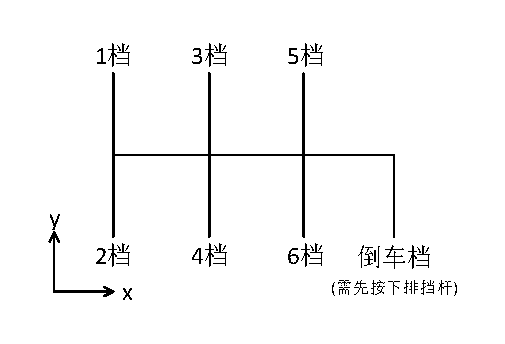
\includegraphics{变速器排挡杆.pdf}
	\caption{变速器排挡杆}
	\label{fig:gearLever}
\end{figure}

该控制逻辑应用于六档变速杆,支持下压式倒挡,其档位映射如图\ref{fig:gearLever}所示。现要求实现相关函数完成图\ref{fig:gearLever}所示控制逻辑,代码应遵循如下要求:

\begin{enumerate}
	\item 该函数应接受4个参数:$ x $、$ y $、$ diverse $和$ oldGear $,根据参数计算出档位值$ gear $并返回;
	\item 返回的档位值$ gear $的取值集合为$\left\{0, 1, 2, 3, 4, 5, 6, -1, -2\right\}$。其中1-6为前进档,-2为倒车档;
	\item $ x $为变速器挡杆在水平方向上的行程。当取值在[0, 380)区间时,表示1或2档;当取值在[380, 690]区间时,表示3或4档;当取值大于690时,表示5、6或-2档(倒车档);
	\item  $ y $为变速器挡杆在竖直方向上的行程。当取值在[0, 160)区间时,档位的可能取值为2、4、6档和-2档;当取值在[160, 780]区间时,档位的可能取值为0或-1(要求下压挡杆);当取值大于780时,档位的可能取值为1、3和5档;
	\item $ diverse $为倒挡信号,当下压变速器挡杆时$ diverse $值为1,否则为0;
	\item $ oldGear $的取值为本次变速器挡杆操作前的档位取值。
\end{enumerate}

\begin{lstlisting}[label=code:gearLever,caption=变速器档位控制的一个函数实现]
int calculateGear(uint x, uint y, uint diverse, int oldGear)
{
	int gear = 0;
	if (y < 160) {
		if (x < 380)
			gear = 2;
		else if (x > 690)
			gear = 6;
		else
			gear = 4;
	}
	else if (y > 780) {
		if (x < 380)
			gear = 1;
		else if (x > 690)
			gear = 5;
		else
			gear = 3;
	}
	if (diverse) {
		if ((gear == 6) && ((oldGear == -1 || oldGear == -2)))
			gear = -2;
		else if (gear == 0);
			gear = -1;
		}
	return gear;
}
\end{lstlisting}

如代码\ref{code:gearLever}所示为上述需求所对应的一个函数实现。当参数取值情况多种多样、条件分支复杂时,开发人员将难以直观的获取到输入输出之间的关系。例如,在需求文档中,档位值为6的条件是$  (x > 690 ∧ y < 160 ∧ (diverse = 0 ∨ (oldGear ≠ -1 ∧ oldGear ≠ -2))) $,但开发者很难直观从代码中获取到相应的控制条件,只有通过表达式分析,才可以自动从代码中得知。试想,如果纯人工的完成这样的行为,不仅费时费力还可能出现条件遗漏和边界条件错误等情况。
更重要的是,因为人工操作的不稳定,很难抓住需求和代码实现之间的微小差异。例如,在以上代码中实际存在了一个很严重的语义问题,导致在$ diverse ≠ 0 $的情况下代码执行与预期不符。即使有完整的需求文档与源代码,没有工具支持的情况下对其进行一致性确认也是十分困难的事情。
本章所述工具可以帮助解决以上问题。如表\ref{tab:summaryFromGearLever}的1、3列所示为期望的返回值与控制逻辑,而实际代码的行为如表\ref{tab:summaryFromGearLever}的1、2列所示(方便起见分别将参数$ diverse $和$ oldGear $简写为$ dv $和$ og $)。不难发现程序无法返回$ gear = -2 $且返回值$ gear $与参数$ oldGear $无关,与预期不符。开发人员通过对比2、3列即可确认出该程序行为与需求之间的差异,帮助发现代码问题。该问题的根源在于程序第23行行尾多了一个分号致使控制流出错,经过修改后程序与需求可完全一致。

\begin{longtable}{ccc}
	\caption{根据代码\ref{code:gearLever}生成的函数摘要}
	\label{tab:summaryFromGearLever}  \\ % add \\ command to tell LaTeX to start a new line	
	 
	% Appear table header at the first page as well
	\toprule[1.5pt]	
	{\heiti 返回值} & {\heiti 实际的控制逻辑} & {\heiti 期望的控制逻辑} \\
	\midrule[1pt]
	\endfirsthead
	
	% Appear the table header at the top of every page
	\multicolumn{3}{c}{续表~\thetable\hskip1em 根据代码\ref{code:gearLever}生成的函数摘要}\\
	\toprule[1.5pt]	
	{\heiti 返回值} & {\heiti 实际的控制逻辑} & {\heiti 期望的控制逻辑} \\
	\midrule[1pt]
	\endhead 
	
	% Appear \hline at the bottom of every page
	\hline
	\multicolumn{3}{r}{续下页}
	\endfoot 
	\endlastfoot
	
	% data begins here	
	2 & - & \begin{tabular}[c]{@{}c@{}}$(x > 690) \wedge (y < 160) \wedge $\\ $(og = -2 ∨ og = -1) \wedge (dv ≠ 0)$\end{tabular} \\ 
	-1 & dv ≠ 0 & $(160 ≤ y ≤ 780) \wedge (dv ≠ 0)$ \\ 
	0 & $(160 ≤ y ≤ 780) \wedge (dv = 0)$ & $(160 ≤ y ≤ 780) \wedge (dv = 0)$ \\ 
	1 & $(x < 380) \wedge (y > 780) \wedge (dv = 0)$ & $(x < 380) \wedge (y > 780)$ \\ 
	2 & $(x < 380) \wedge (y < 160) \wedge (dv = 0)$ & $(x < 380) \wedge (y < 160)$ \\ 
	3 & $(380 ≤ x ≤ 690) \wedge (y > 780) \wedge (dv = 0)$ & $(380 ≤ x ≤ 690) \wedge (y > 780)$ \\ 
	4 & $(380 ≤ x ≤ 690) \wedge (y < 160) \wedge (dv = 0)$ & $(380 ≤ x ≤ 690) \wedge (y < 160)$ \\ 
	5 & $(x > 690) \wedge (y > 780) \wedge (dv = 0)$ & $(x > 690) \wedge (y > 780)$ \\ 
	6 & $(x > 690) \wedge (y < 160) \wedge (dv = 0)$ & \begin{tabular}[c]{@{}c@{}}$(x > 690) \wedge (y < 160) \wedge $\\ $(og ≠ -2 \wedge og ≠ -1)$\end{tabular} \\ 
	% more data here
	\bottomrule[1.5pt]
\end{longtable}
%
%\begin{table}[htb]
%	\centering
%	\caption{根据代码\ref{code:gearLever}生成的函数摘要}
%	\label{tab:summaryFromGearLeverxx}
%	\begin{tabular}{|c|c|c|}
%		\hline
%		返回值 & 实际的控制逻辑 & 期望的控制逻辑 \\ \hline
%		-2 & - & \begin{tabular}[c]{@{}c@{}}$(x > 690) \wedge (y < 160) \wedge $\\ $(og = -2 ∨ og = -1) \wedge (dv ≠ 0)$\end{tabular} \\ \hline
%		-1 & dv ≠ 0 & $(160 ≤ y ≤ 780) \wedge (dv ≠ 0)$ \\ \hline
%		0 & $(160 ≤ y ≤ 780) \wedge (dv = 0)$ & $(160 ≤ y ≤ 780) \wedge (dv = 0)$ \\ \hline
%		1 & $(x < 380) \wedge (y > 780) \wedge (dv = 0)$ & $(x < 380) \wedge (y > 780)$ \\ \hline
%		2 & $(x < 380) \wedge (y < 160) \wedge (dv = 0)$ & $(x < 380) \wedge (y < 160)$ \\ \hline
%		3 & $(380 ≤ x ≤ 690) \wedge (y > 780) \wedge (dv = 0)$ & $(380 ≤ x ≤ 690) \wedge (y > 780)$ \\ \hline
%		4 & $(380 ≤ x ≤ 690) \wedge (y < 160) \wedge (dv = 0)$ & $(380 ≤ x ≤ 690) \wedge (y < 160)$ \\ \hline
%		5 & $(x > 690) \wedge (y > 780) \wedge (dv = 0)$ & $(x > 690) \wedge (y > 780)$ \\ \hline
%		6 & $(x > 690) \wedge (y < 160) \wedge (dv = 0)$ & \begin{tabular}[c]{@{}c@{}}$(x > 690) \wedge (y < 160) \wedge $\\ $(og ≠ -2 \wedge og ≠ -1)$\end{tabular} \\ \hline
%	\end{tabular}
%\end{table}

本章接下来的部分主要解释如何自动化实现以上过程。重点介绍值流图构建、语义分析、表达式分析等关键步骤。

\section{基于值流图的程序理解与需求确认方法}
\label{sec:值流图程序理解方法}

本节介绍的方法是一种基于精确值流图的自动化程序分析算法。值流图是对程序的一种数据流表示,可通过基于内存模型的语义分析自动获得。基于值流图可执行多种静态分析算法,得到结构化表示的程序语义,进而进行需求确认。
算法的工作流程如图\ref{fig:流程图}所示,首先借助现有静态分析框架将源代码转化为语义等价的控制流自动机(CFA),根据CFA提供的内存读写信息进一步生成精确值流图(VFG)。在得到VFG后,执行表达式分析算法进而得到变量间的符号表达式关系,最终根据表达式信息生成模块摘要并保存在源文件中。

\begin{figure}[H]
	\centering
	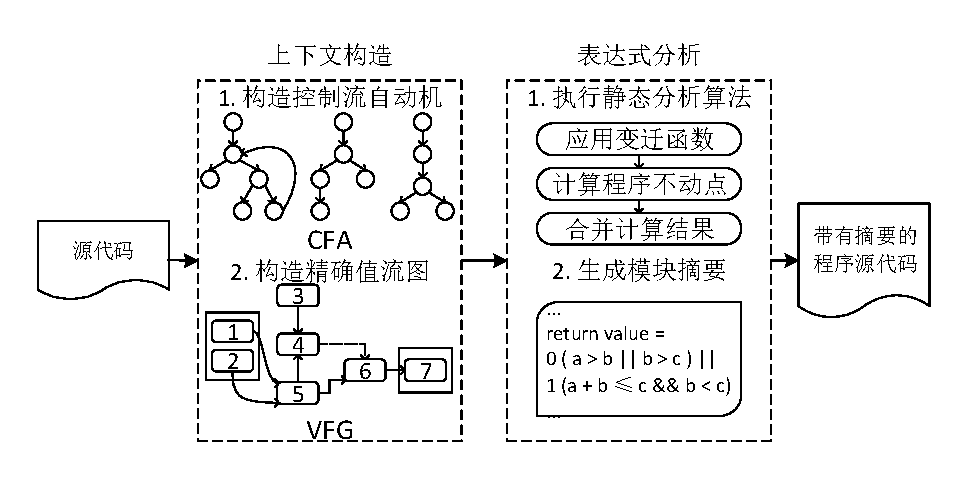
\includegraphics{流程图.pdf}
	\caption{算法的工作流程图}
	\label{fig:流程图}
\end{figure}

\subsection{精确值流图的定义与构造}

在传统的基于控制流图的数据流分析方法中,同一变量在不同路径下的计算结果不同,为了保证算法的正确性,这类算法通常在交汇节点定义状态合并函数,具体使用上近似将变量可能的取值合并。但这将忽略路径信息导致分析精度不足。而精确值流图则是通过内存行为分析与指针别名操作分析,构造出变量取值与数据依赖和控制依赖相结合的值流图。这种精确值流图是路径敏感的,可用来解决状态计算过程中产生的路径丢失问题。

\begin{lstlisting}[label=code:vfgExample,caption=代码样例]
int main() {
	int x = 0, y = 1;
	int *a;
	int p;
	if (p)
		a = &x;
	else
		a = &y;
	return *a;
}
\end{lstlisting}

以代码\ref{code:vfgExample}为例,在第9行的数据流关系为:$ a \gets \{\&x, \&y\} $。而如果使用路径敏感的数据流分析,由于有了路径可达条件信息,可以进一步将a的数据流表示为:$ a \gets \{(\&x, p ≠ 0), (\&y, p = 0)\} $。

\begin{figure}[H]
	\centering
	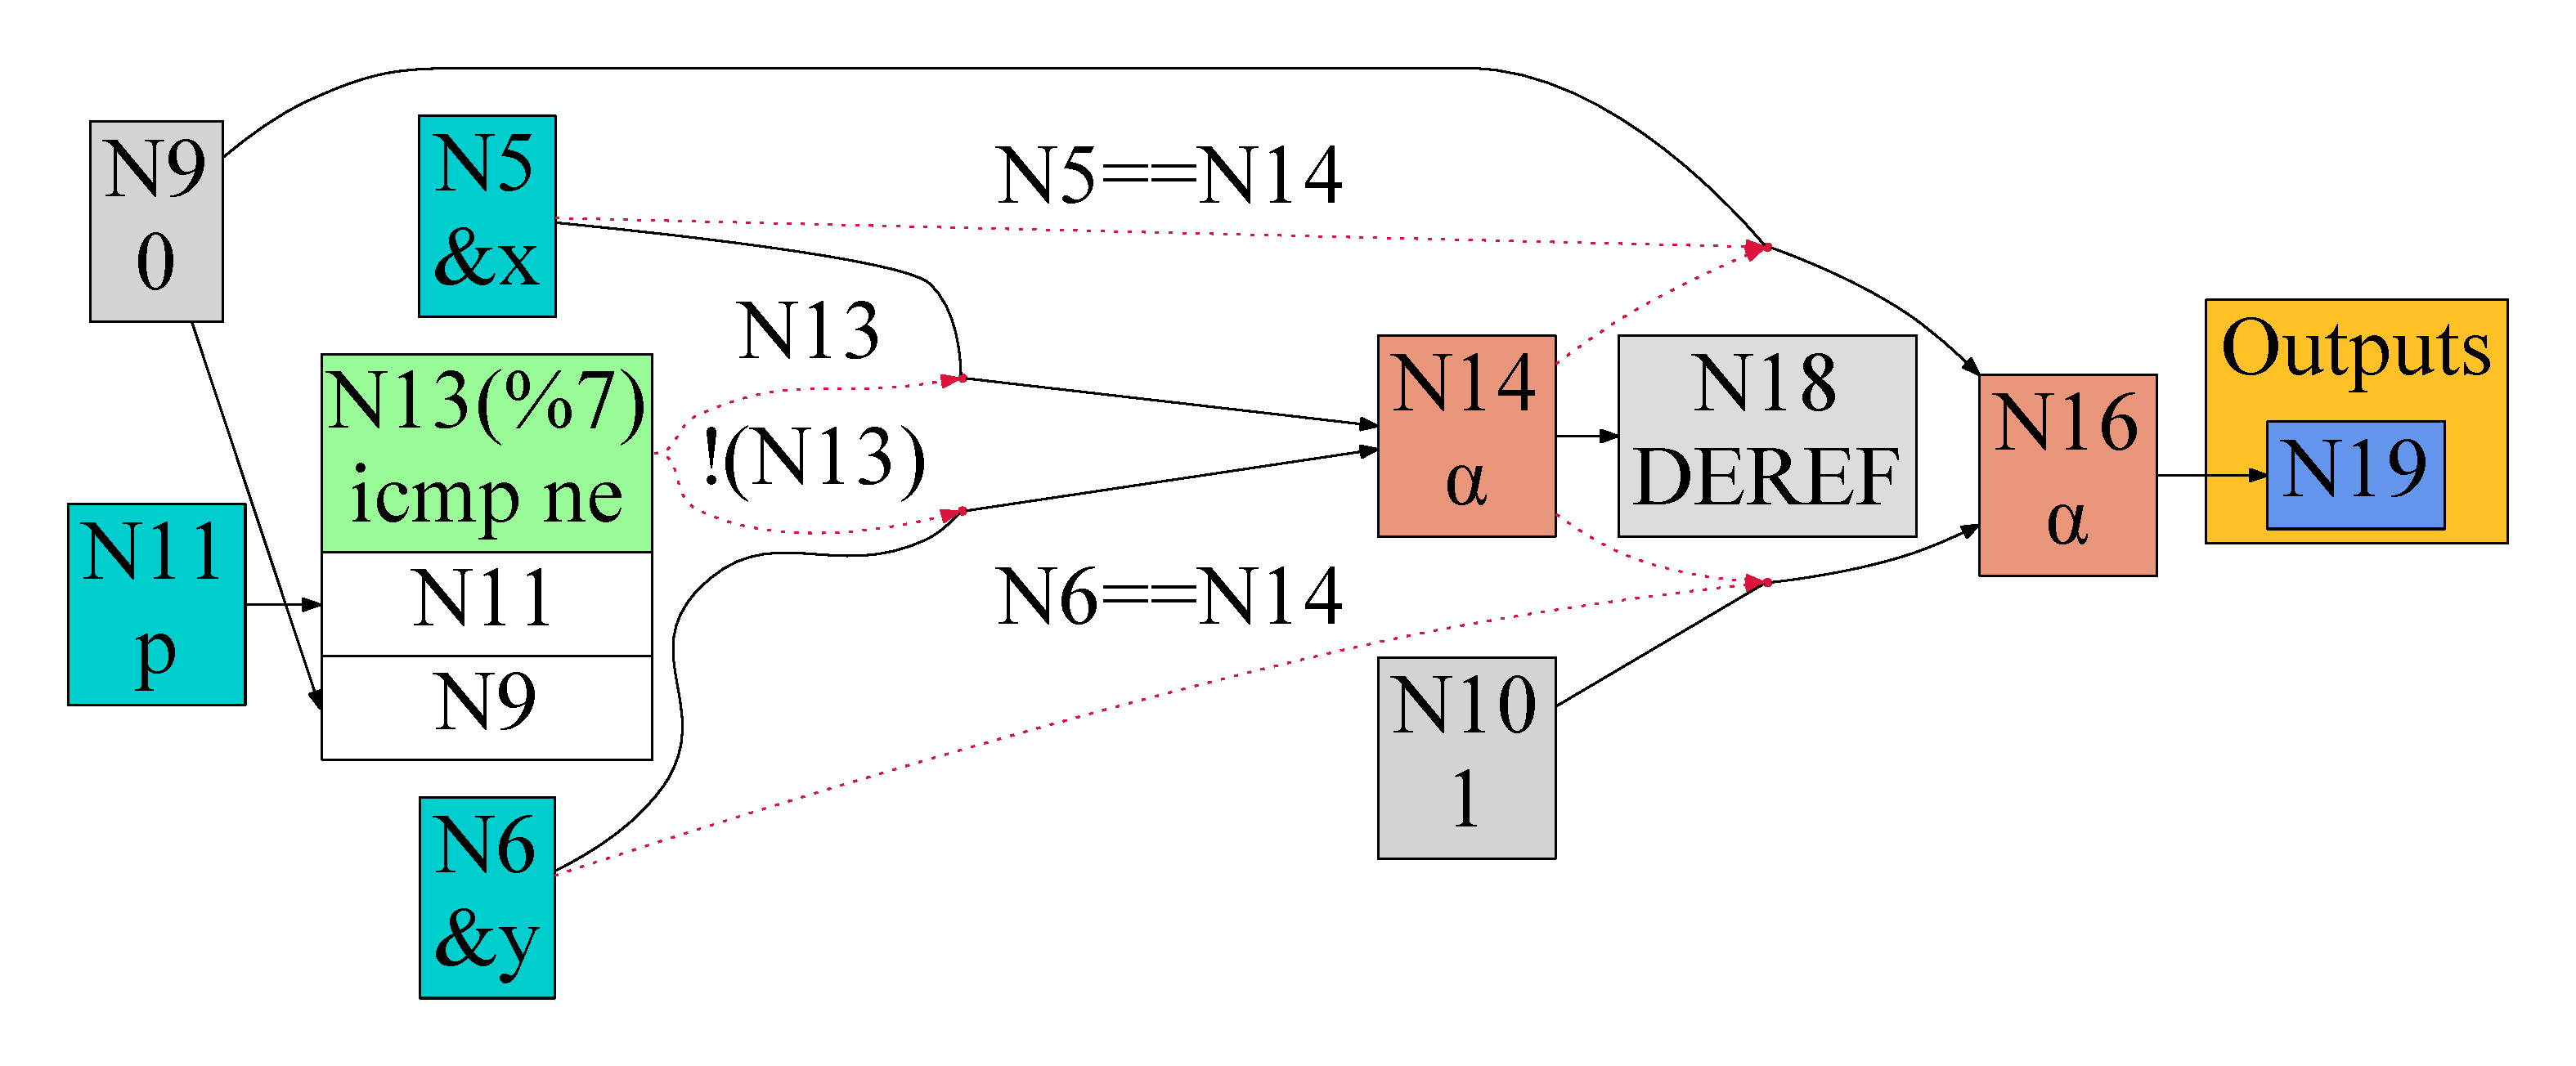
\includegraphics[width=6in]{small.pdf}
	\caption{根据代码\ref{code:vfgExample}生成的值流图}
	\label{fig:small}
\end{figure}

像这样,我们可以把数据流 • ← • 作为值流图上的边,把数据流上承载的数据作为值流图的点,构造值流图如图\ref{fig:small}所示。

值流图按函数划分为不同的值流模块($ Module $),每个$ Module = (N, E) $是一个有向图,其中$ N $是值流图节点集合,每个节点代表程序中的变量或常量。节点$ n ∈ N $上也可以带有条件,表示控制依赖。$ E ⊆ N × N $为有向边集合,表示值的流向。边$ e ∈ E $可以附加条件,表示数据依赖。

我们将VFG的节点按照功能分为如下几类:

常量节点ConstNode:表示程序中的常量,如整数常量、字符串常量、函数指针常量、全局变量的地址常量等,用$ <c> $表示,其中$ c $为字面常量。如图\ref{fig:small}中的节点$ N_{9} $可以表示为$ <0> $。

起始节点StartNode:表示值流图中数据初始化节点,如程序中的变量初始值、参数、函数调用的返回值等等。按照定义可知,起始节点在VFG图中无前驱节点,且该节点不是常量。初始节点用$ <ap> $表示,其中$ ap $是对应的数据的内存位置的访问路径。如图\ref{fig:small}中的节点$ N_{11} $可表示为$ <p> $。

复制节点CopyNode:表示值的复制关系,它的值复制于前驱节点,用$ <n> $表示,其中$ n $是VFG中的节点。如图\ref{fig:small}中的节点$ N_{19} $可表示为$ <N_{16}> $。

运算节点OperatorNode:表示由输入经过运算得到的结果,其中,运算节点以其前驱节点作为运算的输入。运算节点用$ <op, op_1, …, op­_n> $表示,其中$ op $为运算符,$ op_1, …, op­_n $为操作数。这里,操作数即为运算节点的前驱节点。图\ref{fig:small}中节点$ N_{13} $可表示为$ <≠, N_{11}, N_{9}> $。

合并节点JoinNode:合并节点具有多个前驱节点,该节点的取值为前驱节点中的某一个。合并节点用$ <(N_1, C_1), …, (N_i, C_i)> $表示,其中$ N_i $为JoinNode的前驱节点,$ C_i $为数据依赖,表示当$ C_i $为真时,JoinNode的取值为$ N_i $。图\ref{fig:small}中节点$ N_{14} $可表示为$ <(N_5, N_{13}), (N_6, ¬N_{13})> $。

对于每个模块$ M $,定义两个特殊节点集合$ In(M) $和$ Out(M) $分别表示模块的输入节点集合和输出节点集合。其中,输入节点包括函数的参数与全局变量,其类型总是StartNode。而输出节点包括函数的返回值与全局变量,其类型总是CopyNode。

为了便于后续描述算法,我们定义如下函数:
\begin{enumerate}
	\item 定义函数$ literalVal::ConstNode \rightarrow Value $用于取常量节点的具体值;
	\item 定义函数$ symbolicVal::StartNode \rightarrow Value $表示取起始节点的符号值。
\end{enumerate}

\subsection{表达式分析算法}

定义$ ValueCase $为二元组$  (Value, Condition) $,其中$ Value $是值流图上某节点的可能取值,这个值既可以是具体的常量值,如123、“abc”等,又可以是符号表达式,如“a + 3”等;$ Condition $是布尔表达式,它表示当值流图上某节点的$ Condition $条件为真时,其取值为$ Value $。

定义函数$ val::ValueCase \rightarrow Value $表示取$ ValueCase $中$ Value $的值;函数$ cond::ValueCase \rightarrow Condition $表示取$ ValueCase $中$ Condition $的值。

定义抽象函数$ T::Node \rightarrow ValueSet $为从值流图节点到抽象域上的一个映射,其中$ ValueSet $为$ ValueCase $的集合。则基于值流图的表达式分析算法如算法\ref{alg:值流图分析算法}所示。

\begin{algorithm}
[H]
	\caption{值流图分析算法}
	\label{alg:值流图分析算法}
	\begin{algorithmic}[1]
		
		\Require $nodes$: current value flow graph's node set
		
		\State $blockSet \gets \emptyset$
		\State $pending \gets \left\{ n \;|\; n \in nodes, n \text{ is ConstNode or StartNode }\right\}$
		\While{$pending \ne \emptyset$}
		\State $cur \gets $ peek($pending$)
		\State $valueSet \gets$ updateNodeValue($cur$)
		\If{$valueSet = \emptyset$}
		\State $blockSet \gets blockSet \cup cur$
		\ElsIf{$valueSet$ is an update for $cur$}
		\State $pending \gets pending \cup successor(cur)$
		\State move each $node$ from $blockSet$ to $pending$ which is unblocked due to $valueSet$
		\EndIf
		\EndWhile
		
	\end{algorithmic}
\end{algorithm}

其中,函数$ updateNodeValue::Node \rightarrow ValueSet $表示在迭代计算过程中每个节点的计算值,针对不同类型的节点,我们定义不同计算方法,具体计算方法如表\ref{tab:valueUpdate}所示。

\begin{longtable}{cc}
	\caption{各类节点的值的更新算法}
	\label{tab:valueUpdate}  \\ % add \\ command to tell LaTeX to start a new line	
	
	% Appear table header at the first page as well
	\toprule[1.5pt]	
	{\heiti 节点类型} & {\heiti 更新值}  \\
	\midrule[1pt]
	\endfirsthead
	
	% Appear the table header at the top of every page
	\multicolumn{2}{c}{续表~\thetable\hskip1em 各类节点的值的更新算法}\\
	\toprule[1.5pt]	
	{\heiti 节点类型} & {\heiti 更新值}  \\
	\midrule[1pt]
	\endhead 
	
	% Appear \hline at the bottom of every page
	\hline
	\multicolumn{2}{r}{续下页}
	\endfoot 
	\endlastfoot
	
	% data begins here	
	
	ConstNode & $ \left\{ \left( literalVal \left( cur \right), true \right) \right\} $ \\ 
	StartNode & $ \left\{ \left( symbolicVal \left( cur \right), true \right) \right\} $ \\
	CopyNode & $ \left\{ \left(updateNodeValue \left( cur.predecessor \right) \right) \right\} $ \\ 
	OperatorNode &
			$ \left\{ 
					\left( 	\begin{array}{lr}	 		
							operatorValue \\
							\left( opr \left( cur \right), val \left( opd_1 \right), ..., val \left( opd_i \right) \right) \\
							, cond \left( opd_1 \right) \wedge ... \wedge cond \left( opd_i \right) \\
					\end{array} \right)  
			\,\middle\vert\,
					\begin{array}{c}
							opd_i \in T \left( pre_i \right), \\
							pre_i = pred \left( cur \right) \left[ i \right]  
					\end{array}
			\right\} $ \\ 
	JoinNode (Loop) & 
			$ \left\{ \left( \mu, true \right) 
			\,\middle\vert\, 
			\mu \gets \mu \cup val \left( pred \left( cur \right) \right) \right\} $ \\ 
	JoinNode (Normal) & 
			$ \left\{ \left( val \left( pre_i \right), cond \left( pre_i \right) \wedge pcond \left( pre_i \right) \right)
			\,\middle\vert\, 
			pre_i \gets pred_i \left( cur \right) \right\} $ \\ 
	% more data here
	\bottomrule[1.5pt]
\end{longtable}
%
%\begin{table}[htb]
%	\centering
%	\caption{各类节点的值的更新算法}
%	\label{tab:valueUpdatexx}
%	\begin{tabular}{|c|c|}
%		\hline
%		节点类型 & 更新值 \\ \hline
%		ConstNode & $ \left\{ \left( literalVal \left( cur \right), true \right) \right\} $ \\ \hline
%		StartNode & $ \left\{ \left( symbolicVal \left( cur \right), true \right) \right\} $ \\ \hline
%		CopyNode & $ \left\{ \left(updateNodeValue \left( cur.predecessor \right) \right) \right\} $ \\ \hline
%		OperatorNode &
%				$ \left\{ 
%					 		\left( 	\begin{array}{lr}	 		
%							 		operatorValue \\
%							 		\left( opr \left( cur \right), val \left( opd_1 \right), ..., val \left( opd_i \right) \right) \\
%							 		, cond \left( opd_1 \right) \wedge ... \wedge cond \left( opd_i \right) \\
%					 		\end{array} \right)  
%				 		\,\middle\vert\,
%				 				\begin{array}{c}
%				 						opd_i \in T \left( pre_i \right), \\
%				 						pre_i = pred \left( cur \right) \left[ i \right]  
%				 				\end{array}
%				\right\} $ \\ \hline
%		JoinNode (Loop) & 
%				$ \left\{ \left( \mu, true \right) 
%				\,\middle\vert\, 
%				\mu \gets \mu \cup val \left( pred \left( cur \right) \right) \right\} $ \\ \hline
%		JoinNode (Normal) & 
%				$ \left\{ \left( val \left( pre_i \right), cond \left( pre_i \right) \wedge pcond \left( pre_i \right) \right)
%				\,\middle\vert\, 
%				pre_i \gets pred_i \left( cur \right) \right\} $ \\ \hline
%	\end{tabular}
%\end{table}

本算法属于值流图分析算法,定义了两个集合$ pending $和$ blockSet $,分别用于分别用于存储分析算法中待分析的节点和被阻塞的节点。

算法初始化时,将$ blockSet $集合置空,并将所有类型为$ StartNode $和$ ConstNode $的节点置入$ pending $集合中。在每次迭代计算过程中,从$ pending $集合中取出一个节点,如果其前驱节点或数据依赖条件没有计算完成,则将该节点放入$ pending $集合中;否则,按照上表所规定的计算规则对该节点进行计算。如果之前从未对该节点进行过计算,或计算结果与之前不同,则将该节点的全部后继节点放入$ pending $集合中,并检查$ blockSet $中是否有依赖于本次计算结果的节点可被计算,如果有,则将相应节点重新置入$ pending $集合中。根据上述方法,直到所有的节点均被计算完成、并且到达不动点,迭代结束。

\subsection{程序理解与需求确认}
以变速器档位控制代码(代码\ref{code:gearLever})为例,其对应的值流图如图\ref{fig:test-error}所示。

\begin{figure}[H]
	\centering
	\includegraphics[width=6in]{test-error.pdf}
	\caption{根据代码\ref{code:gearLever}生成的值流图}
	\label{fig:test-error}
\end{figure}

应用上述算法对所有节点进行计算,部分节点的计算结果如表\ref{tab:calculationResult}所示。

由于每个模块的输入节点集合$ In(M) $描述了模块所有可能的读入、输出节点集合$ Out(M) $描述了模块所有可能的输出,因此可根据输出输出节点集合构造函数摘要。如图\ref{fig:test-error}所示,由于$ Out(M) $中的节点$ N_{59} $为复制节点,其计算结果与$ N_{56} $相同,因此最终可以得到的模块摘要如表\ref{tab:summaryFromGearLever}第1、2列所示。

摘要清晰的描述了在不同分支路径条件下模块的输入与输出之间的对应关系,从而便于将软件实现与需求文档进行对比,进而提高程序理解与需求确认等工作的效率。另一方面,本算法是一种基于值流图的程序静态分析方法,因此在得到变量表达式关系的同时,可以在其上应用检查规则从而实现代码检查。典型的应用是检查每个节点在不同程序路径下的取值(表达式),判定程序是否存在如除零异常、空指针解引用、多重内存释放等缺陷,提高代码的正确率。

\begin{longtable}{cc}
	\caption{值流图上部分节点的计算结果}
	\label{tab:calculationResult}  \\ % add \\ command to tell LaTeX to start a new line	
	 
	% Appear table header at the first page as well
	\toprule[1.5pt]	
	{\heiti $Node$} & {\heiti $T(Node)$}  \\
	\midrule[1pt]
	\endfirsthead
	
	% Appear the table header at the top of every page
	\multicolumn{2}{c}{续表~\thetable\hskip1em 值流图上部分节点的计算结果}\\
	\toprule[1.5pt]	
	{\heiti $Node$} & {\heiti $T(Node)$}  \\
	\midrule[1pt]
	\endhead 
	
	% Appear \hline at the bottom of every page
	\hline
	\multicolumn{2}{r}{续下页}
	\endfoot 
	\endlastfoot
	
	% data begins here	
	$ N_{4} $ & $ \left\{  \left( x, true \right) \right\} $ \\ 
	$ N_{26} $ & $ \left\{  \left( 690, true \right) \right\} $ \\ 
	$ N_{34} $ & $ \left\{  \left( x > 690, true \right) \right\} $ \\ 
	$ N_{38} $ & $ \left\{  \left( 4, x ≤ 690 \right), \left( 6, x > 690 \right) \right\} $ \\ 
	$ N_{41} $ & $ \left\{  \left( 1, x < 380 \right), \left( 3, 380 ≤ x ≤ 690 \right), \left( 5, x > 690 \right) \right\} $ \\ 
	$ N_{42} $ & $ \left\{  
			\begin{array}{c}
					\left( 0, y ≤ 780 \right), \left( 1, x < 380 \wedge y > 780 \right) , \left( 3, 380 ≤ x ≤ 690 \wedge y > 780 \right) , \\
					\left( 5, x > 690 \wedge y > 780 \right) 
			\end{array}				
			\right\} $ \\ 
	$ N_{56} $ & $ \left\{  
			\begin{array}{c}
					\left( -1, dv ≠ 0 \right), \left( 0, 160 ≤ y ≤780 \wedge dv = 0 \right), \left( 1, x < 380 ∧ y > 780 \wedge dv = 0 \right),  \\
					\left( 2, x < 380 \wedge y < 160 \wedge dv = 0 \right), \left( 3, 380 ≤ x ≤ 690 \wedge y > 780 \wedge dv = 0 \right),  \\
					\left( 4, 380 ≤ x ≤ 690 \wedge y < 160 \wedge dv = 0 \right), \left( 5, x > 690 \wedge y > 780 \wedge dv = 0 \right), \\
					\left( 6, x > 690 \wedge y < 160 \wedge dv = 0 \right),  \\
			\end{array}
			\right\} $ \\ 
	% more data here
	\bottomrule[1.5pt]
\end{longtable}

%\begin{table}[H]
%	\centering
%	\caption{值流图上部分节点的计算结果}
%	\label{tab:calculationResultxx}
%	\begin{tabular}{|c|c|}
%		\hline
%		$Node$ & $T(Node)$ \\ \hline
%		$ N_{4} $ & $ \left\{  \left( x, true \right) \right\} $ \\ \hline
%		$ N_{26} $ & $ \left\{  \left( 690, true \right) \right\} $ \\ \hline
%		$ N_{34} $ & $ \left\{  \left( x > 690, true \right) \right\} $ \\ \hline
%		$ N_{38} $ & $ \left\{  \left( 4, x ≤ 690 \right), \left( 6, x > 690 \right) \right\} $ \\ \hline
%		$ N_{41} $ & $ \left\{  \left( 1, x < 380 \right), \left( 3, 380 ≤ x ≤ 690 \right), \left( 5, x > 690 \right) \right\} $ \\ \hline
%		$ N_{42} $ & $ \left\{  
%				\begin{array}{c}
%						\left( 0, y ≤ 780 \right), \left( 1, x < 380 \wedge y > 780 \right) , \left( 3, 380 ≤ x ≤ 690 \wedge y > 780 \right) , \\
%						\left( 5, x > 690 \wedge y > 780 \right) 
%				\end{array}				
%		\right\} $ \\ \hline
%		$ N_{56} $ & $ \left\{  
%				\begin{array}{c}
%						\left( -1, dv ≠ 0 \right), \left( 0, 160 ≤ y ≤780 \wedge dv = 0 \right), \left( 1, x < 380 ∧ y > 780 \wedge dv = 0 \right),  \\
%						\left( 2, x < 380 \wedge y < 160 \wedge dv = 0 \right), \left( 3, 380 ≤ x ≤ 690 \wedge y > 780 \wedge dv = 0 \right),  \\
%						\left( 4, 380 ≤ x ≤ 690 \wedge y < 160 \wedge dv = 0 \right), \left( 5, x > 690 \wedge y > 780 \wedge dv = 0 \right), \\
%						\left( 6, x > 690 \wedge y < 160 \wedge dv = 0 \right),  \\
%				\end{array}
%		\right\} $ \\ \hline
%	\end{tabular}
%\end{table}

\section{评估与结果}
\label{sec:值流图评估与结果}

\subsection{实验设计}

虑到根据源代码生成精确值流图的过程十分复杂,本算法的实现基于Tsmart静态分析框架,它的优点是使用静态分析的方法,高效的生成控制流自动机和精确值流图。同时该分析框架具有可配置性,能够较容易的获取到所需程序上下文信息,因此我们采用此分析框架,工具的开发语言为Java,工具的框架图如图\ref{fig:架构图}所示。

本节从客观、主观两个方面评估论文算法(工具)在程序理解与需求确认方面的效用。客观评价重点关注算法的完整性与准确性。具体而言,我们考察算法自动生成的摘要质量;主观评价则重点关注工具在具体的生产环境中的可用性与实用性。我们将分别从客观评价和主观评价两个方面对工具进行实验。

\begin{figure}[H]
	\centering
	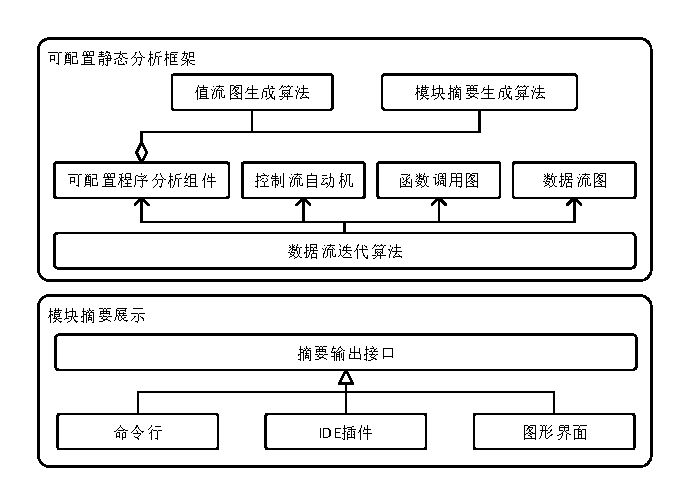
\includegraphics[width=6in]{架构图.pdf}
	\caption{工具架构图}
	\label{fig:架构图}
\end{figure}

\subsection{客观评价}

客观评价方法主要包含以下几个步骤:(1)分别选取数学计算、计算机应用、工业领域和嵌入式领域中8个具有代表性的代码片段作为实验对象(详见表\ref{tab:selectedCodes});(2)采用本文工具分别生成相应的函数摘要;(3)判定工具自动生成的摘要与实际需求的差距。
\begin{longtable}{ccc}
	\caption{选取的各类代码}
	\label{tab:selectedCodes}  \\ % add \\ command to tell LaTeX to start a new line	
	 
	% Appear table header at the first page as well
	\toprule[1.5pt]	
	{\heiti 类别} & {\heiti 选取代码}  & {\heiti 文件名称}  \\
	\midrule[1pt]
	\endfirsthead
	
	% Appear the table header at the top of every page
	\multicolumn{3}{c}{续表~\thetable\hskip1em 选取的各类代码}\\
	\toprule[1.5pt]	
	{\heiti 类别} & {\heiti 选取代码}  & {\heiti 文件名称}  \\
	\midrule[1pt]
	\endhead 
	
	% Appear \hline at the bottom of every page
	\hline
	\multicolumn{3}{r}{续下页}
	\endfoot 
	\endlastfoot
	
	% data begins here	
	\multirow{2}{*}{数学计算} & 三角形判定 & triangle.c \\ 
	& 绝对值计算 & abs.c \\ 
	\multirow{2}{*}{计算机应用} & (加权平均)滤波算法 & filter.c \\ 
	& 校验和算法 & checksum.c \\ 
	\multirow{2}{*}{工业领域} & 车辆控制系统某算法 & CDL\_ARC429.c \\ 
	& 航天发动机控制系统某算法 & ISP\_TOOL.c \\
	\multirow{2}{*}{嵌入式领域} & 含goto语句的程序片段 & msp430-decode.c \\
	& 带函数指针的程序片段 & xen-ops.c \\ 
	% more data here
	\bottomrule[1.5pt]
\end{longtable}
%\begin{table}[htb]
%	\centering
%	\caption{选取的各类代码}
%	\label{tab:selectedCodesxx}
%	\begin{tabular}{|c|c|c|}
%		\hline
%		类别 & 选取代码 & 文件名称 \\ \hline
%		\multirow{2}{*}{数学计算} & 三角形判定 & triangle.c \\ \cline{2-3} 
%		& 绝对值计算 & abs.c \\ \hline
%		\multirow{2}{*}{计算机应用} & (加权平均)滤波算法 & filter.c \\ \cline{2-3} 
%		& 校验和算法 & checksum.c \\ \hline
%		\multirow{2}{*}{工业领域} & 车辆控制系统某算法 & CDL\_ARC429.c \\ \cline{2-3} 
%		& 航天发动机控制系统某算法 & ISP\_TOOL.c \\ \hline
%		\multirow{2}{*}{嵌入式领域} & 含goto语句的程序片段 & msp430-decode.c \\ \cline{2-3} 
%		& 带函数指针的程序片段 & xen-ops.c \\ \hline
%	\end{tabular}
%\end{table}

由于摘要结果和程序的条件分支有关,因此本文分别对比两者在每个条件分支下的生成结果。同时,记录工具的时间和空间开销,包括摘要生成时间、占用内存大小以及生成的VFG大小,如表\ref{tab:summaryComparision}所示。

\begin{table}[htb]
	\centering
	\caption{自动生成摘要和人工生成摘要的对比}
	\label{tab:summaryComparision}
	\begin{tabular}{|c|c|c|c|c|c|c|c|}
		\hline
		\multicolumn{2}{|c|}{程序代码} & 实际需求 & \multicolumn{4}{c|}{自动摘要} & \multirow{2}{*}{\begin{tabular}[c]{@{}c@{}}正确\\ 率\end{tabular}} \\ \cline{1-7}
		类型 & 代码行 & 分支数 & 分支数 & 耗时/s & 内存/MB & VFG大小/KB &  \\ \hline
		三角形判定 & 24 & 4 & 4 & 3 & 134 & 9 & 1.0 \\ \hline
		绝对值 & 11 & 2 & 2 & 2 & 122 & 2 & 1.0 \\ \hline
		滤波算法 & 19 & 1 & 1 & 2 & 128 & 4 & 1.0 \\ \hline
		校验和算法 & 22 & 1 & 1 & 2 & 145 & 12 & 1.0 \\ \hline
		车辆控制系统 & 124 & 12 & 12 & 5 & 167 & 53 & 1.0 \\ \hline
		航发控制系统 & 178 & 15 & 15 & 6 & 171 & 61 & 1.0 \\ \hline
		Goto语句 & 57 & 8 & 8 & 4 & 137 & 34 & 1.0 \\ \hline
		函数指针 & 36 & 3 & 3 & 3 & 132 & 6 & 1.0 \\ \hline
	\end{tabular}
\end{table}

经实验验证,本工具能够完整地生成不同类型代码的摘要,且生成摘要的条件分支数与需求一致。运行工具所消耗的资源相对较少,内存占用小于200MB,生成的VFG均小于1MB。工具可以较快的生成函数摘要,生成百行级别代码所需时间不超过1分钟。

\subsection{主观评价}

为保证主观评价的公平性与准确性,现从学校选取共30名条件相当的同学参与实验,他们均符合以下条件:(1)拥有超过3年的C语言编程经验,且均使用C语言通过了学校的编程水平测验;(2)对表\ref{tab:selectedCodes}代码所在的背景了解程度相当。

实验方法包含以下几个步骤:(1)将30名同学分为源码组和摘要组进行对照实验,分别为其提供表5所示的8份源代码(或含摘要的源代码);(2)令每名同学阅读代码,并令其说出代码功能,记录用时T1;(3)令每名同学分析函数在不同输入的情况下的输出,记录用时T2;(4)分别统计并对比两组同学在不同代码上回答问题所用时间T1和T2的平均值;(5)在源码组同学完成后,为其提供摘要。同时分别询问两组同学对摘要的看法。 

如表\ref{tab:ComprehensionComparision}所示为两组同学在各个代码上回答实验步骤2和3中提出问题的平均用时T1和T2。通过对比可知,在代码行数较小(10行以内)且逻辑并不复杂的情况下,使用摘要对程序理解无明显帮助。但当面对几十甚至上百行代码时,使用摘要可明显减少用户理解代码所用时间。在含goto语句的实验样本上,可节省60.5\%的程序理解时间。

通过实验可知,本工具可显著提高用户对代码的理解效率,能够帮助用户快速抽取程序语义并进行需求确认。同时,随着代码分支复杂度的提升,使用工具进行程序理解与需求确认的优势将越来越大。

\begin{longtable}{ccccc}
	\caption{各组对每类代码理解并作答所用时间}
	\label{tab:ComprehensionComparision}  \\ % add \\ command to tell LaTeX to start a new line	

	% Appear table header at the first page as well
	\toprule[1.5pt]	
	{\heiti 程序代码} & {\heiti 源码组T1/s}  & {\heiti 源码组T2/s}  & {\heiti 摘要组T1/s}  & {\heiti 摘要组T2/s}    \\
	\midrule[1pt]
	\endfirsthead
	
	% Appear the table header at the top of every page
	\multicolumn{5}{c}{续表~\thetable\hskip1em 选取的各类代码}\\
	\toprule[1.5pt]	
	{\heiti 程序代码} & {\heiti 源码组T1/s}  & {\heiti 源码组T2/s} & {\heiti 摘要组T1/s}   & {\heiti 摘要组T2/s}    \\
	\midrule[1pt]
	\endhead 
	
	% Appear \hline at the bottom of every page
	\hline
	\multicolumn{5}{r}{续下页}
	\endfoot 
	\endlastfoot
	
	% data begins here	
	三角形判定 & 45 & 32 & 37 & 14 \\ 
	绝对值 & 5 & 13 & 11 & 14 \\ 
	滤波算法 & 61 & 15 & 27 & 15 \\ 
	校验和算法 & 97 & 43 & 54 & 38 \\ 
	车辆控制系统 & 294 & 86 & 103 & 74 \\ 
	航发控制系统 & 318 & 92 & 114 & 91 \\ 
	Goto语句 & 195 & 48 & 64 & 31 \\ 
	函数指针 & 82 & 33 & 40 & 29 \\ 
	% more data here
	\bottomrule[1.5pt]
\end{longtable}
%\begin{table}[htb]
%	\centering
%	\caption{各组对每类代码理解并作答所用时间}
%	\label{tab:ComprehensionComparisionxx}
%	\begin{tabular}{|c|c|c|c|c|}
%		\hline
%		程序代码 & 源码组T1/s & 源码组T2/s & 摘要组T1/s & 摘要组T2/s \\ \hline
%		三角形判定 & 45 & 32 & 37 & 14 \\ \hline
%		绝对值 & 5 & 13 & 11 & 14 \\ \hline
%		滤波算法 & 61 & 15 & 27 & 15 \\ \hline
%		校验和算法 & 97 & 43 & 54 & 38 \\ \hline
%		车辆控制系统 & 294 & 86 & 103 & 74 \\ \hline
%		航发控制系统 & 318 & 92 & 114 & 91 \\ \hline
%		Goto语句 & 195 & 48 & 64 & 31 \\ \hline
%		函数指针 & 82 & 33 & 40 & 29 \\ \hline
%	\end{tabular}
%\end{table}

在实验步骤5中,我们设计了数道问题,交予参与实验的同学回答并统计,最终得到的结果如表\ref{tab:questionaire}。实验参与者对自动生成摘要工具总体持肯定态度,认为生成的摘要对理解代码有帮助。对于摘要是否可以帮助分析变更影响范围与帮助软件维护方面,一部分同学持观望和怀疑态度,认为本工具生成的摘要为函数级别的摘要,而变更影响范围分析与软件维护可能涉及全局代码,需要结合函数调用等信息进一步分析。

\begin{longtable}{cccc}
	\caption{问卷设计与答复情况}
	\label{tab:questionaire}  \\ % add \\ command to tell LaTeX to start a new line	
	
	% Appear table header at the first page as well
	\toprule[1.5pt]	
	{\heiti 问题设计} & {\heiti 赞同人数}  & {\heiti 否定人数}  & {\heiti 其他想法}  \\
	\midrule[1pt]
	\endfirsthead
	
	% Appear the table header at the top of every page
	\multicolumn{4}{c}{续表~\thetable\hskip1em 问卷设计与答复情况}\\
	\toprule[1.5pt]	
	{\heiti 问题设计} & {\heiti 赞同人数}  & {\heiti 否定人数}  & {\heiti 其他想法}  \\
	\midrule[1pt]
	\endhead 
	
	% Appear \hline at the bottom of every page
	\hline
	\multicolumn{4}{r}{续下页}
	\endfoot 
	\endlastfoot
	
	% data begins here	
	摘要是否有助于你理解代码? & 28 & 2 & 0 \\
	你认为摘要是否对影响范围分析有帮助? & 25 & 4 & 1 \\ 
	你认为摘要是否对软件维护有帮助? & 22 & 7 & 1 \\ 
	% more data here
	\bottomrule[1.5pt]
\end{longtable}
%\begin{table}[htb]
%	\centering
%	\caption{问卷设计与答复情况}
%	\label{tab:questionairexx}
%	\begin{tabular}{|c|c|c|c|}
%		\hline
%		问题设计 & 赞同人数 & 否定人数 & 其他想法 \\ \hline
%		摘要是否有助于你理解代码? & 28 & 2 & 0 \\ \hline
%		你认为摘要是否对影响范围分析有帮助? & 25 & 4 & 1 \\ \hline
%		你认为摘要是否对软件维护有帮助? & 22 & 7 & 1 \\ \hline
%	\end{tabular}
%\end{table}

\section{后续工作与总结}
\label{sec:值流图总结}

本方法依赖于精确值流图的准确生成,当前可用工具相对较少,且在面对大型程序时消耗的时间空间较多。这会对本工具的结果造成一定影响。一个可能的解决方案是在原有的值流图算法上进行优化,针对于循环与数组,优化其结果。

另一方面,为了保证算法的收敛性与时间开销,本算法在处理循环时,引入了符号值$ \mu $,算法的结果是带$ \mu $的符号表达式,这将在处理循环时带来一定的精度丢失。后续可以使用循环不变式等技术进一步提高分析精度。同时,为了增强工具对全局影响范围的分析,后续将会结合函数调用等信息,提升工具的适用性。

软件验证与维护是软件研发中不可或缺的一环,而提高研发者对程序的理解速度则是其中的关键所在。传统的技术和工具或者难以有效帮助程序员减少代码阅读量,或者具有较高的使用门槛,难以广泛使用。本文的研究工作试图针对这一问题,提供一个程序理解算法与摘要生成工具。

本章首先通过一个变速器档位控制逻辑的案例剖析了程序理解对软件开发的重要性,并借此提出函数摘要的作用。随后介绍相关程序理解方法与摘要生成算法。我们在可配置的静态分析框架上实现了摘要生成算法,并从内外两个方面结合实验证明了摘要生成算法的有效性与实用性。

尽管本章提出的方法具有一定的局限性,但本章的研究结果仍可对程序理解、变量表达式分析和程序变更影响分析工具的设计与实现提供思路和指导。
% !TeX root = ../main.tex

\chapter{总结与展望}

\section{工作总结}

软件验证与软件确认一直是软件研发过程中不可或缺且十分重要的步骤。本文围绕软件验证与确认在生产实践中面临的两类具体问题提出了有针对性的解决方案。其一,针对当前线性区间抽象域因表示能力不足而造成的程序分析精度损失的问题,本文提出了基于位敏感的区间代数的整型缺陷检测方法。它提高了当前区间抽象域的表示能力,且在保证分析效率的情况下提升了分析精度;其二,针对当前软件确认过程中因程序理解困难而造成的工作低效问题,本文提出了基于精确值流图的整型变量关系分析与缺陷检测方法。借助生成的模块摘要,研发人员可方便的确认程序语义与需求是否相符,发现细微的语义差异,可有效提升程序理解效率并进一步应用于缺陷分析。总体上,本文完成了如下工作内容:

\begin{enumerate}
	\item 基于位敏感的区间代数的整型缺陷检测方法。为了实现这一目标,本文首先进行了线性区间理论域的设计,设计的核心目标有两点,其一是增加表示符号性的能力,其二是将单独区间表示改换为多区间表示。为此,本文依次定义了线性区间Range、线性多区间MultiRange以及位敏感的线性多区间SignRange。通过定义理论域、设计计算规则并优化特定情况下的运算,SignRange能够较好的表示程序中整型变量的可能取值范围。另一方面,为了实现程序语义的表示与分析,本文定义了区间状态RangeState来描述程序的每个状态,通过设计抽象域与变迁规则,实现对程序状态变迁的模拟,从而实现程序的语义分析。最后,通过设计RangeState上的缺陷检测规则,实现了程序的整型缺陷检测。
	
	\item 基于精确值流图的程序理解与需求确认方法。为了实现这一目标,本文首先通过一个具体案例,分析了程序的摘要对程序理解的帮助。本文对精确值流图的定义和构造方法做出了说明,并基于精确值流图,设计了程序语义的抽取方法。具体地,本文完成了关于变量表达式的抽象域的设计、变迁规则的设计与表达式分析算法的设计。在上述的基础上,实现对程序整型变量在不同程序路径下取值关系的语义抽取。最后,借助得到的语义信息生成模块摘要。
	
	\item 模块实现。在提出以上两点的问题解决方案后,本文对其中提到的方法进行了编码实现。基于Tsmart-V3静态分析框架所提供的完备的函数接口,可以方便的获取如控制流自动机、精确值流图等信息。通过编程得到相应工具后,本文设计了一系列的实验,通过实验验证了工具、算法的有效性与实用性。
\end{enumerate}

目前,本文的部分工作已集成至Tsmart-V3工具中,并成功应用于某研究所的生产研发环节。在其自主研发的操作系统上,应用Tsmart已成功帮助其确认了代码中存在的缺陷,具有较好的实际应用价值。

\section{研究展望}

在现有研究工作内容的基础上,为了进一步提高分析的效率和精度,可以针对如下两个方面展开工作:

\begin{enumerate}
	\item 优化位敏感区间的抽象表示。在\ref{sec:SignRange}小节中,为了实现对整型变量符号性的抽象表示,本文定义了符号性Signedness理论域,并结合线性多区间,对程序中具有符号性意义的整型变量提供了抽象表示。但这对理论域的编码实现带来了困难:试想,一个具有符号性的整型变量,其在计算机上的存储内容对固定值而言是不变的,但本文提出的抽象域对同一数值依据不同符号性构造了有符号和无符号两个不同的抽象表示,并设计了算法在其之间做符号性的转化。为了优化位敏感区间的抽象表示方法,我们可以设计新的理论域:这个理论域可以忠实于整型变量在计算机上的二进制串表示,并设计解析规则,对同一个表示整型数值的二进制串根据其符号性不同而使用不同的解析方式,从而得到具体的整数值。这样做所带来的好处是可以进一步减少程序分析所消耗的内存以及更加便于编码实现。
	
	\item 优化程序分析中对循环的处理方式。在\ref{sec:区间算数评估与结果}小节和\ref{sec:值流图评估与结果}小节中,造成工具在实验中产生误报的原因均由程序分析在循环上的处理策略造成。为了追求静态分析精度与效率的平衡,现有技术通常采用循环不变式技术来计算程序在循环中的行为。为了进一步优化现有分析精度,应分别对整型分析与变量表达式分析这两个模块在循环不变式上的计算方式做优化。
\end{enumerate}


%软件的验证与确认在软件研发过程中一直是重点关注的内容。本文聚焦于帮助开发人员快速发现并定位软件中可能存在的数值导向型缺陷,以及
%
%减少软件验证中存在的困难,同时通过
%
%同时聚焦于帮助软件维护人员解决软件确认过程中程序理解困难的问题,从而加速软件确认工作的效率。
%
%提出了基于精确值流图的程序理解与需求确认方法。总体上,本文完成了以下工作内容:
%
%\begin{enumerate}[1)]
%	\item 设计并实现了线性区间理论域,它以区间的形式刻画了C语言整型变量的可能取值范围。主要解决的技术难点是线性区间理论域的设计。
%\end{enumerate}
%
%
%其核心是理论域的设计。本章先介绍了整体的区间设计,随后依次对各个抽象层面进行介绍,并结合控制流自动机,设计了整型变量的缺陷检测规则。最后,在基于Tsmart-V3静态分析框架上做了实现,并通过实验验证了其有效性。
%
%在\ref{sec:Integer}小节,我们介绍了扩展的整数RangeInteger,相比于整数,其具体定义了$ +\infty $和$ -\infty $的概念,同时,我们介绍了有$ -\infty, +\infty $参与的整数运算规则,为后续介绍区间抽象域奠定了基础。在\ref{sec:Range}小节,介绍了基于扩展整数的区间Range,它以单独区间的形式表示了一个整型变量的可能取值范围,并首次定义整数区间上的运算规则。
%
%随后,在\ref{sec:MultiRange}和\ref{sec:SignRange}小节,我们介绍了线性多区间MultiRange与位敏感的线性多区间SignRange,它们的提出分别解决了单独的Range区间精度不足以及无法描述符号性的问题。随后为了进一步提升多区间在区间长度较小时的精度,提出了基于拆分-合并思想的精度提升方法。
%
%最后,结合CPA,提出了基于区间算数的缺陷检测方法。该方法基于区间状态RangeState抽象域,它是CFA上程序状态节点的抽象。通过设计抽象域与变迁规则,可以得到整型变量在程序指令执行前后的取值区间,从而实现整型缺陷分析,并通过实验验证了有效性。
%
%在实验中,测试用例的误报主要原自基于for循环的检测。由于循环摘要的精度受制于循环不变式技术,为了进一步提升整型缺陷分析在循环中的精度,后续的工作重点将集中在循环不变式上。


% 其它部分
\backmatter

%% 本科生要求的几个索引。
% \listoffigures    % 插图索引
% \listoftables     % 表格索引
% \listofequations  % 公式索引

% 参考文献
\bibliographystyle{thuthesis-numeric}      % 顺序编码制
% \bibliographystyle{thuthesis-author-year}  % 著者-出版年制
% \bibliographystyle{thuthesis-bachelor}     % 本科生参考文献的著录格式
\bibliography{ref/refs}

% 致谢
% !TeX root = ../main.tex

\begin{acknowledgements}
	
	衷心感谢顾明老师,周旻老师的指导。
	
\end{acknowledgements}


% 声明
\statement

% 附录
\appendix
% \input{data/appendix-survey}       % 本科生:外文资料的调研阅读报告
% \input{data/appendix-translation}  % 本科生:外文资料的书面翻译
% \input{data/appendix}

% 个人简历
% !TeX root = ../main.tex

\begin{resume}

  \resumeitem{个人简历}

  1995 年 3 月 6 日出生于 内蒙古莫力达瓦自治旗。

  2013 年 9 月考入 大连理工大学 软件学院 软件工程专业,2017 年 7 月本科毕业并获得软件工程学士学位。

  2017 年 9 月考研进入 清华大学 软件学院 攻读 软件工程硕士学位至今。

  \researchitem{发表的学术论文} % 发表的和录用的合在一起

%  % 1. 已经刊载的学术论文(本人是第一作者,或者导师为第一作者本人是第二作者)
%  \begin{publications}
%    \item Yang Y, Ren T L, Zhang L T, et al. Miniature microphone with silicon-
%      based ferroelectric thin films. Integrated Ferroelectrics, 2003,
%      52:229-235. (SCI 收录, 检索号:758FZ.)
%    \item 杨轶, 张宁欣, 任天令, 等. 硅基铁电微声学器件中薄膜残余应力的研究. 中国机
%      械工程, 2005, 16(14):1289-1291. (EI 收录, 检索号:0534931 2907.)
%    \item 杨轶, 张宁欣, 任天令, 等. 集成铁电器件中的关键工艺研究. 仪器仪表学报,
%      2003, 24(S4):192-193. (EI 源刊.)
%  \end{publications}

  % 2. 尚未刊载,但已经接到正式录用函的学术论文(本人为第一作者,或者
  %    导师为第一作者本人是第二作者)。
  \begin{publications}[before=\publicationskip,after=\publicationskip]
    \item Li Wu, Zhou Min, Huang Hao. Program Understanding and Requirement Validation Based on Accurate Value Flow Graph. (已被 WCSE 2020 录用.  )
  \end{publications}

%  % 3. 其他学术论文。可列出除上述两种情况以外的其他学术论文,但必须是
%  %    已经刊载或者收到正式录用函的论文。
%  \begin{publications}
%    \item Wu X M, Yang Y, Cai J, et al. Measurements of ferroelectric MEMS
%      microphones. Integrated Ferroelectrics, 2005, 69:417-429. (SCI 收录, 检索号
%      :896KM)
%    \item 贾泽, 杨轶, 陈兢, 等. 用于压电和电容微麦克风的体硅腐蚀相关研究. 压电与声
%      光, 2006, 28(1):117-119. (EI 收录, 检索号:06129773469)
%    \item 伍晓明, 杨轶, 张宁欣, 等. 基于MEMS技术的集成铁电硅微麦克风. 中国集成电路,
%      2003, 53:59-61.
%  \end{publications}

%  \researchitem{研究成果} % 有就写,没有就删除
%  \begin{achievements}
%    \item 任天令, 杨轶, 朱一平, 等. 硅基铁电微声学传感器畴极化区域控制和电极连接的
%      方法: 中国, CN1602118A. (中国专利公开号)
%  \end{achievements}

\end{resume}


% 本科生的综合论文训练记录表
% \includepdf[pages=-]{scan-record.pdf}

\end{document}
